\chapter{\textbf{Test Results \& Discussions}}
\begin{justify}
From experimental data, various calculations were performed using ‘MATLAB’ environment. The Digital Signal Analysis- Toolbar is a great tool for signal processing and smoothing. As the data were some arbitrary thus a processing is needed to overcome the problem. Mainly Fast Fourier Transformations were performed for better signal processing. The below figures are the results:
\end{justify}
\section{Sensor Signal Analysis \& Processing}

From experimental data, various calculations were performed using ‘MATLAB’ environment. The Digital Signal Analysis- Toolbar is a great tool for signal processing and smoothing. As the data were some arbitrary thus a processing is needed to overcome the problem. Mainly Fast Fourier Transformations were performed for better signal processing. The below figures are the results:
\begin{enumerate}[label=\roman*]
\setlength{\parskip}{0.0pt}
\item \textbf{Coherence Estimation via Welch Method:}In digital signal processing, coherence is a statistics between two functions or
signals which is used to estimate the power transfer of the input and output in a linear/linear time-invariant system. This algorithm is based on standard MATLAB’s tools. The standard derivation of the mean is computed as \cite{sethi2017internet,tsang2017iot,zawawi2018electromyography,gres2019orthogonal,regalia2018adaptive,de2013inverse,cohen2018automated,van2018signal,anchal2018nonlinearity,seichter2018online,lewicki2009eddy,hijazi2018ambient};\par


\begin{equation}\tag{7.1}
 \sigma  ( f ) = \sqrt[]{\frac{2}{N \vert  \Upsilon  ( f ) ^{2} \vert } ( 1- \vert  \Upsilon  ( f )  \vert ^{2} ) ^{2}}
\end{equation}
\begin{justify}
Where,
\end{justify}


\begin{equation}\tag{7.2}
 \vert  \Upsilon  ( f )  \vert ^{2}= \frac{ \vert P_{xy} ( f )  \vert ^{2}}{P_{xx} ( f ) .P_{yy} ( f ) }
\end{equation}
\begin{justify}
Is the coherence function.In signal processing, the coherence is a statistic that can be used to examine the relation between two signals or data sets. It is commonly used to estimate the power transfer between input and output of a linear system. If the signals are ergodic, and the system function linear, it can be used to estimate the causality between the input and output.The computed coherence (Figure 7.1) indicates that at most of the major ocean tidal frequencies the variation of groundwater level at this particular site is over 90\% due to the forcing of the ocean tides. However, one must exercise caution in attributing causality. If the relation (transfer function) between the input and output is nonlinear, then values of the coherence can be erroneous. Another common mistake is to assume a causal input/output relation between observed variables, when in fact the causative mechanism is not in the system model. By using equations-(7.1) $\&$  (7.2), Figure-7.1, can be plotted. Here, Figure-7.1 depicts the coherence estimation via Welch method. This figure shows that no data has been overlapped into one another.
\end{justify}

\begin{figure}[H]
	\begin{Center}
		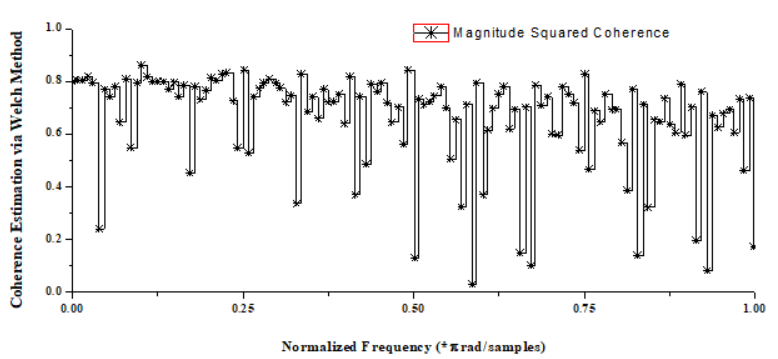
\includegraphics[width=6in,height=2in]{15}
		\caption{ Coherence estimation via Welch method }
		\label{fig:_1_Coherence_estimation_via_Welch_method_}
	\end{Center}
\end{figure}


%%%%%%%%%%%%%%%%%%%% Figure/Image No: 24 Ends here %%%%%%%%%%%%%%%%%%%%

\par

\setlength{\parskip}{8.04pt}
\par

\setlength{\parskip}{0.0pt}
The Figure 7.2, denotes the magnitude response curve. The rms signal-to-noise ratio for an ideal N-bit converter is:\par


\begin{equation}\tag{7.3}
Signal to Noise Ratio (SNR) = 20log_{10}\frac{r.m.s value of F_{s} input}{r.m.s value of quantization noise}
\end{equation}

\begin{equation}\tag{7.4}
or, SNR = 20log_{10}\frac{q^{2^{N}}/2\sqrt[]{2}}{q/\sqrt[]{2}}=20log_{10}2^{N}+20log_{10}\sqrt[]{\frac{3}{2}}
\end{equation}
\begin{justify}
SNR = 6.02N + 1.76 dB (13), over the Nyquist bandwidth of interest.
\end{justify}\par



%%%%%%%%%%%%%%%%%%%% Figure/Image No: 25 starts here %%%%%%%%%%%%%%%%%%%%

\begin{figure}[H]
	\begin{Center}
		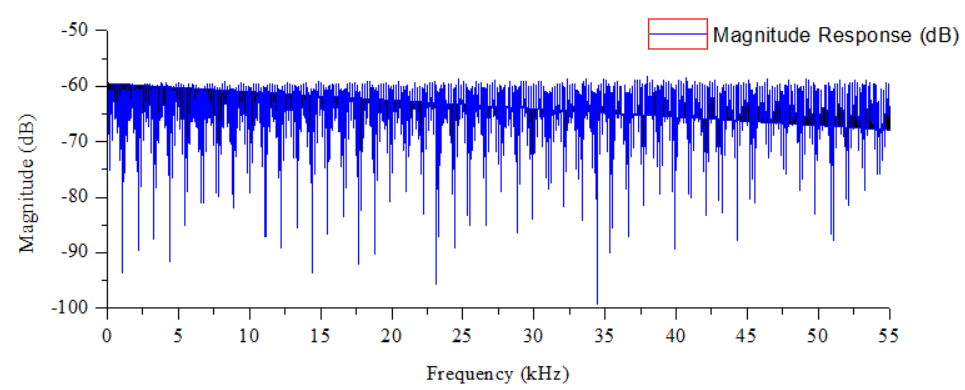
\includegraphics[width=5.91in,height=2.16in]{16}
		\caption{ Magnitude Response Graph (Gas Sensor)}
		\label{fig:_2_Magnitude_Response_Graph_Gas_Sensor}
	\end{Center}
\end{figure}
 The transfer function is independent of the spectral properties of the stimulus as long as the system behaves linearly and as long as the input and output signals are measured at sufficient SNR.

%%%%%%%%%%%%%%%%%%%% Figure/Image No: 25 Ends here %%%%%%%%%%%%%%%%%%%%

\par

\par

\begin{justify}
Figure 7.3, represents the combination of magnitude and phase response. The plot shows limited errors.
\end{justify}\par



%%%%%%%%%%%%%%%%%%%% Figure/Image No: 26 starts here %%%%%%%%%%%%%%%%%%%%

\begin{figure}[H]
	\begin{Center}
		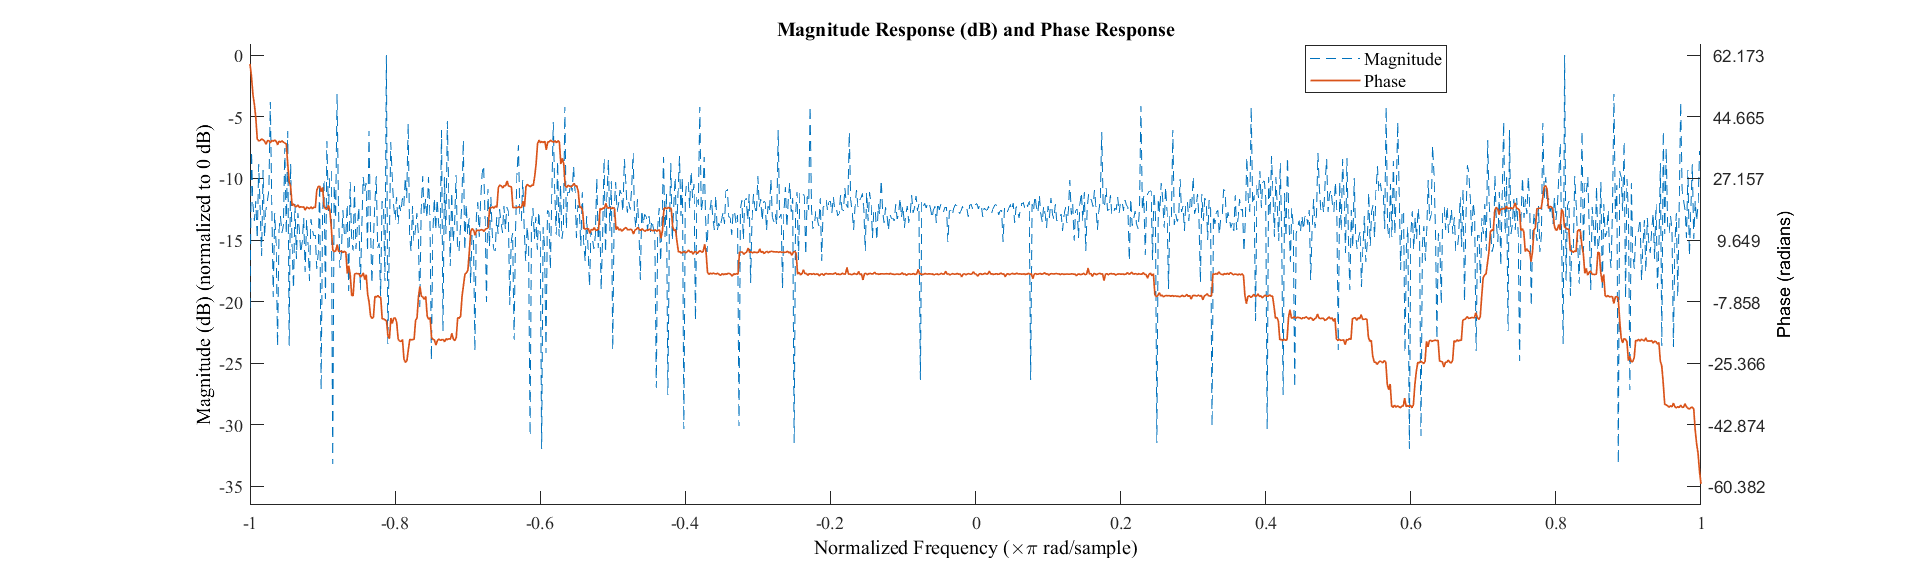
\includegraphics[width=5.52in,height=2.73in]{17}
		\caption{ Magnitude and Phase Response (Gas Sensor) }
		\label{fig:_3_Magnitude_and_Phase_Response_Gas_Sensor_}
	\end{Center}
\end{figure}


%%%%%%%%%%%%%%%%%%%% Figure/Image No: 26 Ends here %%%%%%%%%%%%%%%%%%%%

\par

\par

\item \textbf{Time Domain signal processing:} Now, using the gas sensor data Time-domain graph was plotted in Figure-7.4 to Figure-7.7,
along with a 3rd and 8\textsuperscript{th} order Fast Fourier Transformation (FFT) of the signal for better analysis. The Fourier series is a sum of sine and cosine functions that describes a periodic signal. It is represented in either the trigonometric form or the exponential form. The toolbox provides this trigonometric Fourier series form [45]:\par


\begin{equation}\tag{7.5}
y=a_{0}+ \sum _{i=1}^{n}a_{i}cos ( iwx ) +b_{i}sin ( iwx )
\end{equation}
\setlength{\parskip}{8.04pt}
where a\textsubscript{0} models a constant (intercept) term in the data and is associated with the i = 0 cosine term, w is the fundamental frequency of the signal, n is the number of terms (harmonics) in the series, and 1 $ \leq $  n $ \leq $  8.Time domain refers to the analysis of mathematical functions, physical signals or time series of economic or environmental data, with respect to time. In the time domain, the signal or function's value is known for all real numbers, for the case of continuous time, or at various separate instants in the case of discrete time. An oscilloscope is a tool commonly used to visualize real-world signals in the time domain. A time-domain graph shows how a signal changes with time, whereas a frequency-domain graph shows how much of the signal lies within each given frequency band over a range of frequencies. A Savitzky–Golay filter is a digital filter that can be applied to a set of digital data points for the purpose of smoothing the data, that is, to increase the signal-to-noise ratio without greatly distorting the signal. This is achieved, in a process known as convolution, by fitting successive sub-sets of adjacent data points with a low-degree polynomial by the method of linear least squares. Figure-7.4 depicts the plots of Raw analog, Savitzky Golay Filtered value, moving avg. filtered value and the median plot.\par



%%%%%%%%%%%%%%%%%%%% Figure/Image No: 27 starts here %%%%%%%%%%%%%%%%%%%%

\begin{figure}[H]
	\begin{Center}
		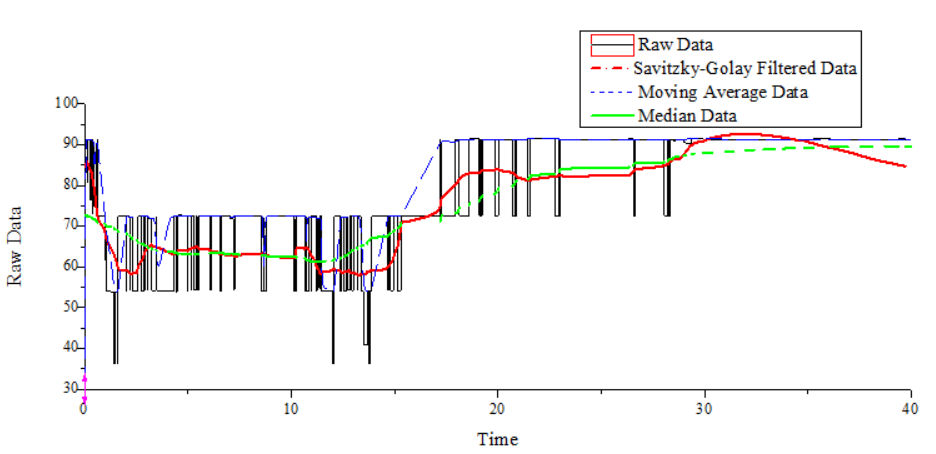
\includegraphics[width=6.5in,height=2.72in]{18}
		\caption{Processed Signal (PPM vs Time)}
		\label{fig:_4_Processed_Signal_PPM_vs_Time}
	\end{Center}
\end{figure}


%%%%%%%%%%%%%%%%%%%% Figure/Image No: 27 Ends here %%%%%%%%%%%%%%%%%%%%

\setlength{\parskip}{0.0pt}
\par

\par


\vspace{\baselineskip}

\vspace{\baselineskip}

\vspace{\baselineskip}
\begin{justify}
Figure 7.5 shows the Furrier fitted curve for gas sensor value.
\end{justify}\par



%%%%%%%%%%%%%%%%%%%% Figure/Image No: 28 starts here %%%%%%%%%%%%%%%%%%%%

\begin{figure}[H]
  \centering
  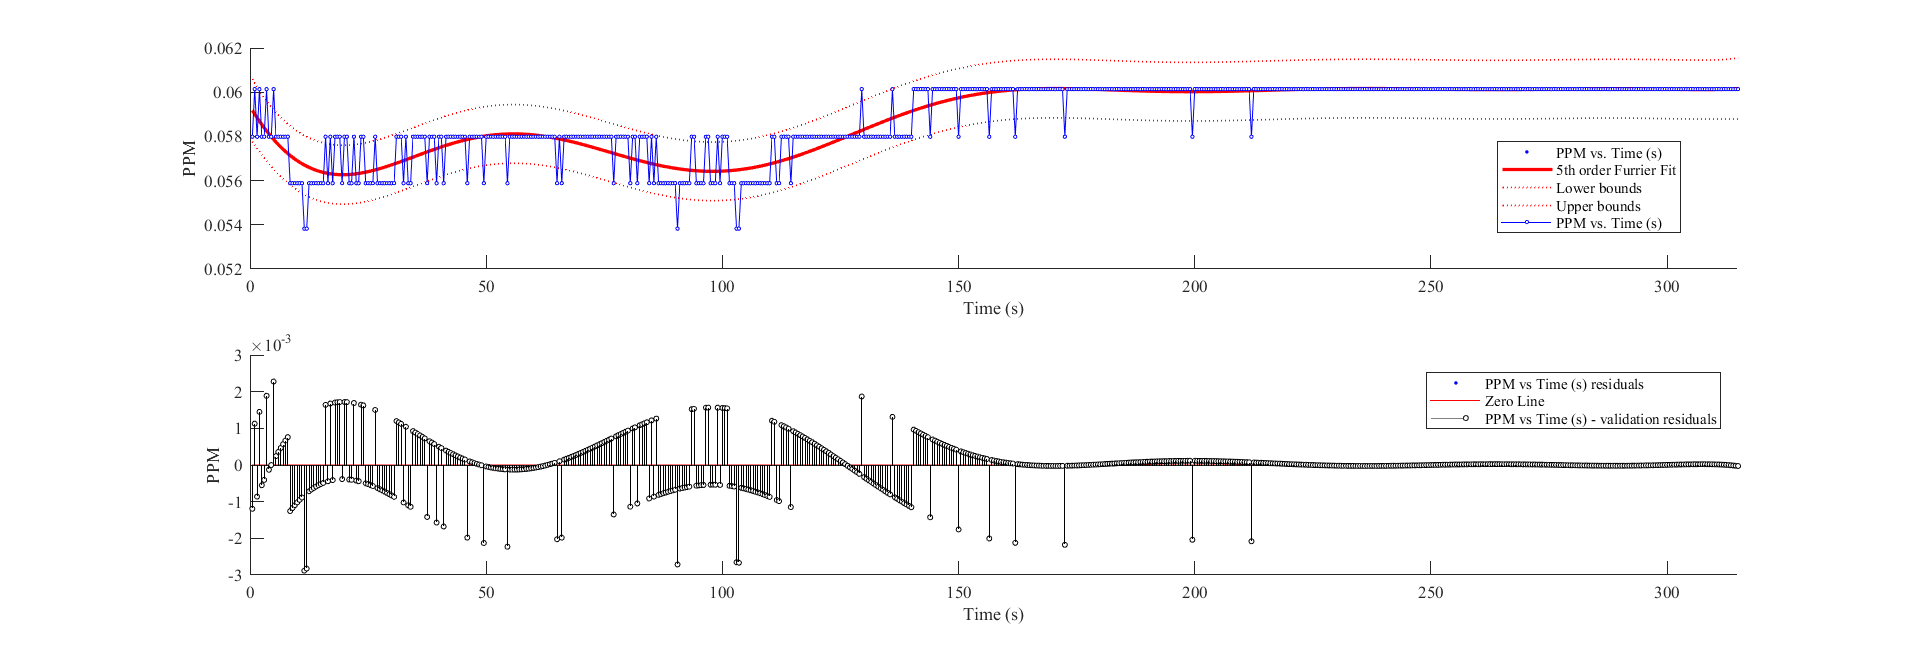
\includegraphics[width=6.5in,height=2.38in]{19}
  \caption{Furrier fitted curve for gas sensor value}\label{fig19}
\end{figure}
%\begin{figure}[H]
%	\begin{Center}
%		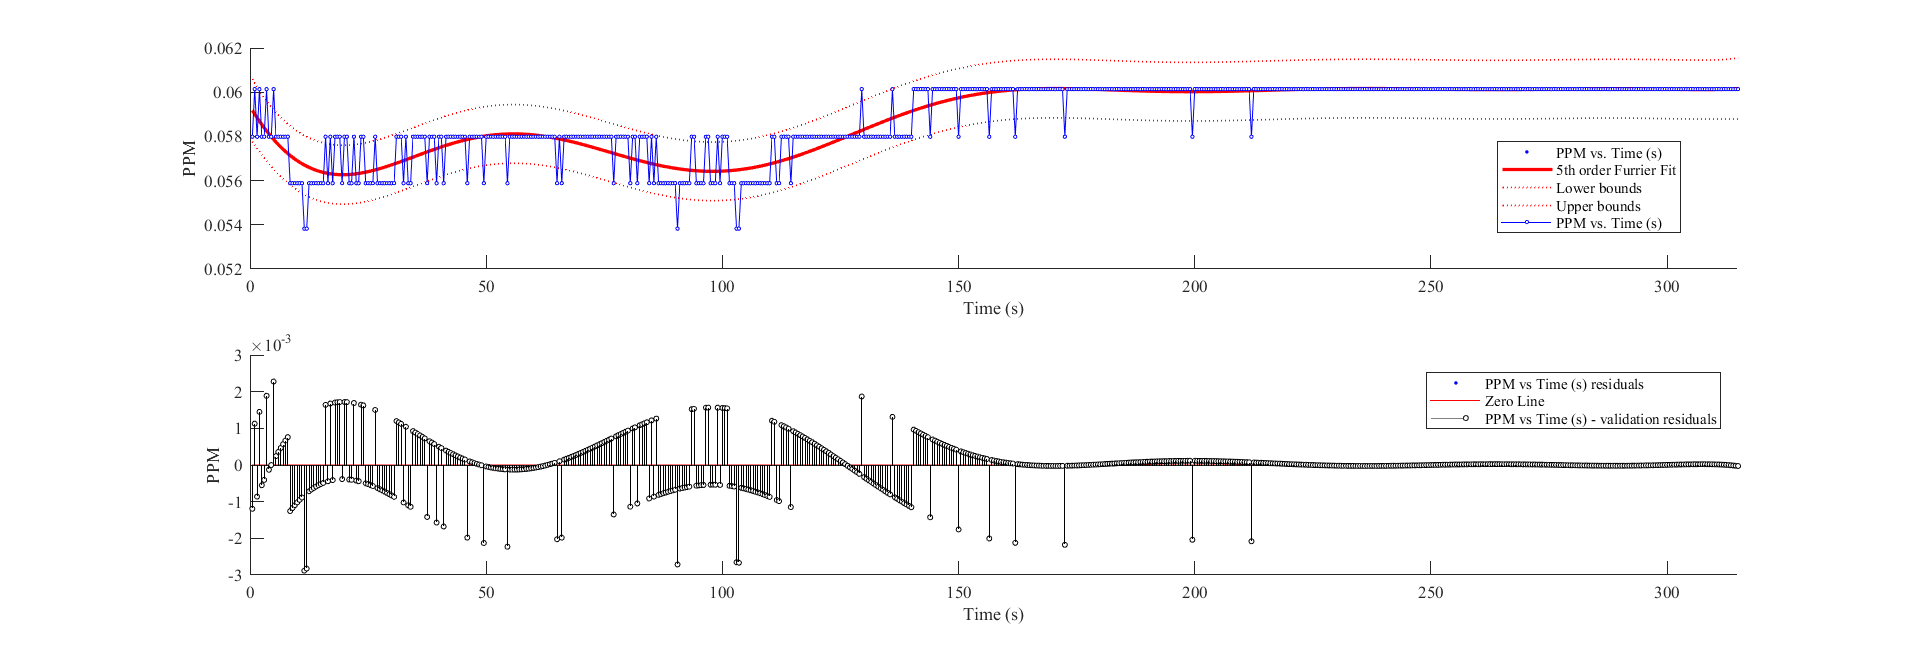
\includegraphics[width=6.5in,height=2.38in]{19}
%	\end{Center}
%\end{figure}


%%%%%%%%%%%%%%%%%%%% Figure/Image No: 28 Ends here %%%%%%%%%%%%%%%%%%%%

\par

\par


\vspace{\baselineskip}
\begin{justify}
The below Figure 7.6 $\&$  7.7 are the same plots as Figure 7.4 $\&$  7.5, but those value represents the Temperature and Humidity.
\end{justify}\par



%%%%%%%%%%%%%%%%%%%% Figure/Image No: 29 starts here %%%%%%%%%%%%%%%%%%%%

\begin{figure}[H]
	\begin{Center}
		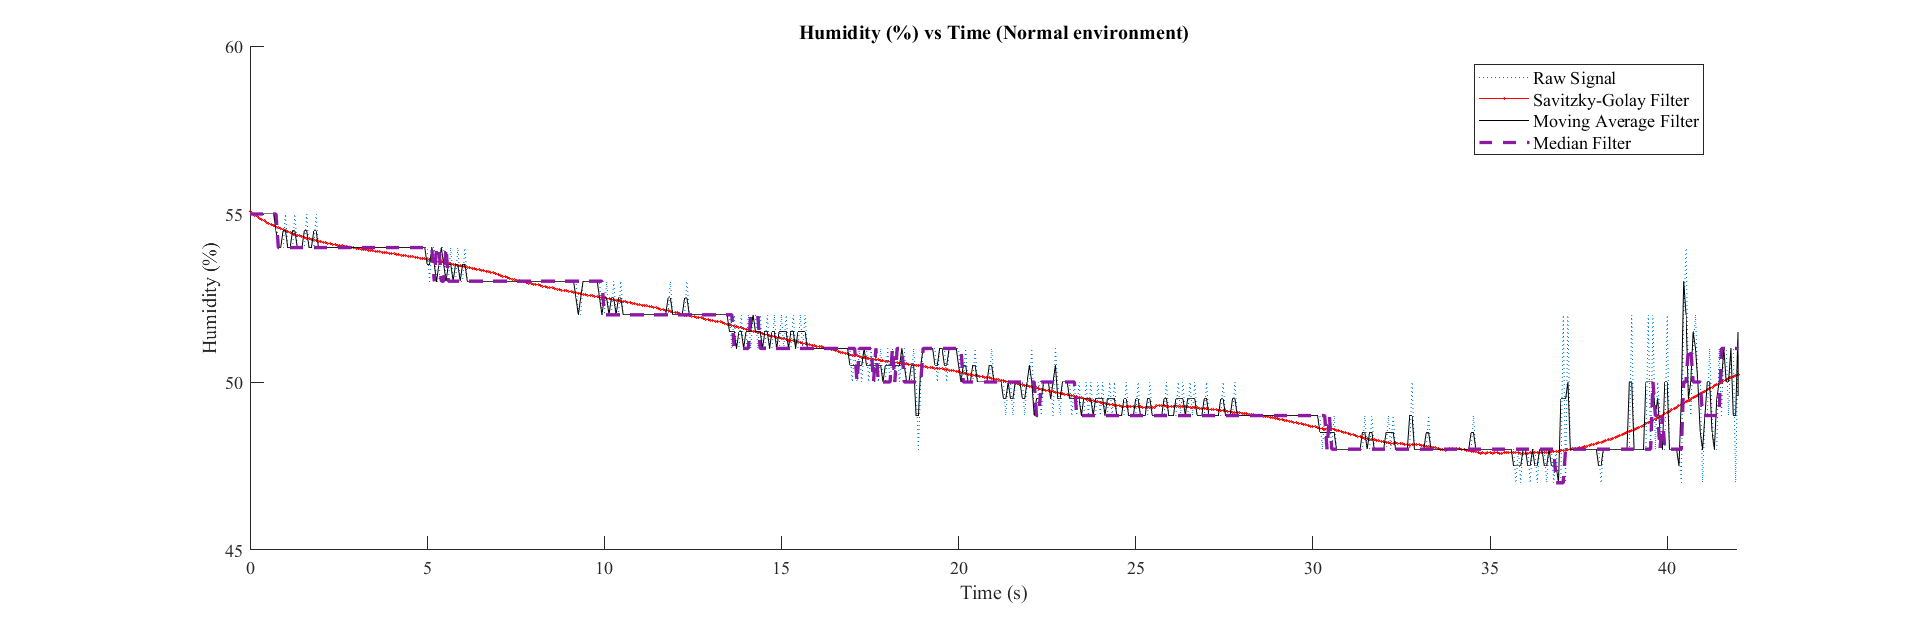
\includegraphics[width=6.36in,height=2.81in]{20}
		\caption{Processed Signal (Humidity vs Time)}
		\label{fig:_6_Processed_Signal_Humidity_vs_Time}
	\end{Center}
\end{figure}


%%%%%%%%%%%%%%%%%%%% Figure/Image No: 29 Ends here %%%%%%%%%%%%%%%%%%%%

\par

\par


\vspace{\baselineskip}


%%%%%%%%%%%%%%%%%%%% Figure/Image No: 30 starts here %%%%%%%%%%%%%%%%%%%%

\begin{figure}[H]
	\begin{Center}
		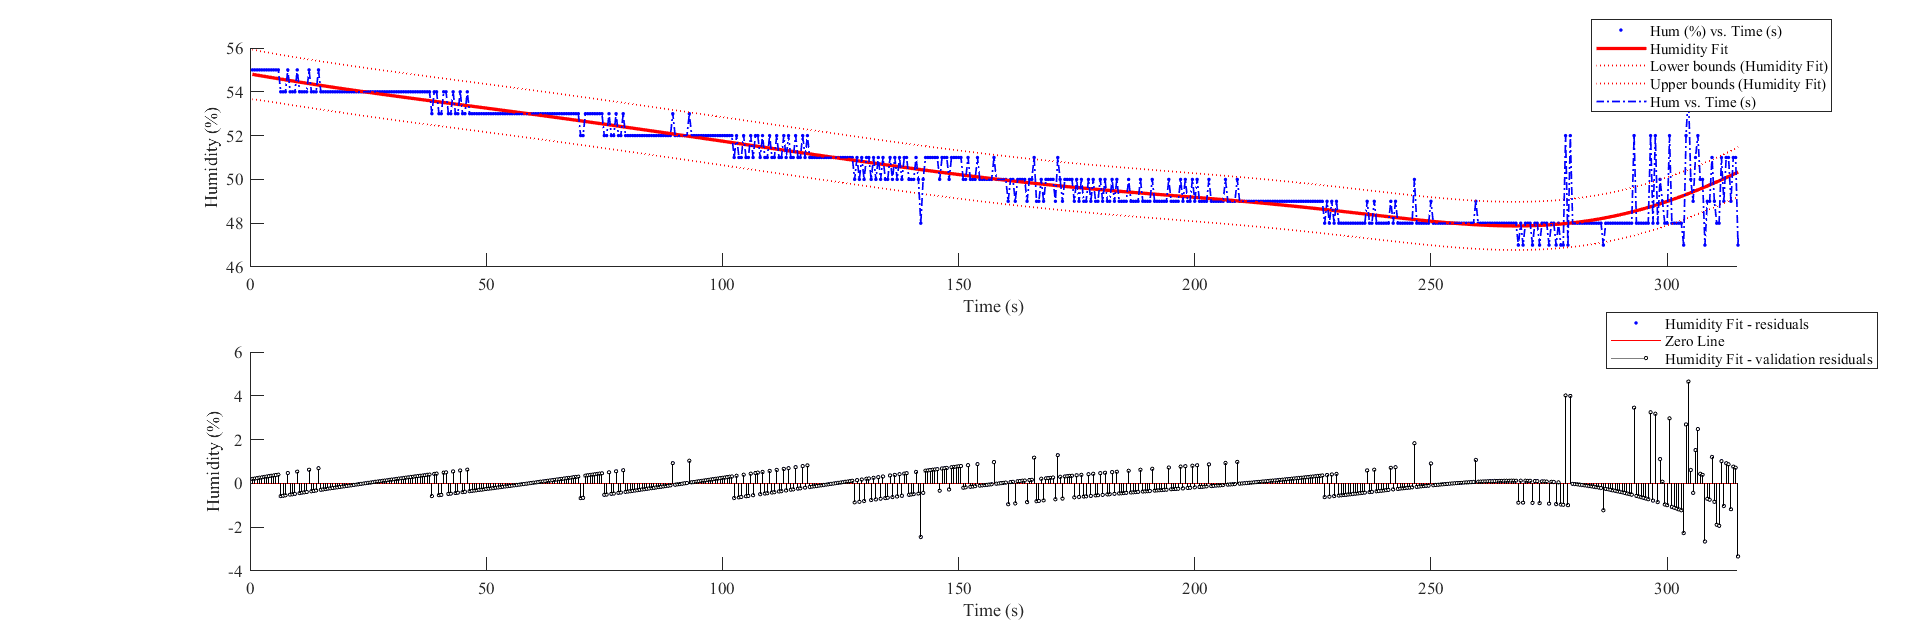
\includegraphics[width=6.25in,height=3.47in]{21}
	\end{Center}
\caption{Humidity vs Time domain graph with $8^{th}$ order furrier transform using 95\% of confidence limit}
\end{figure}


%%%%%%%%%%%%%%%%%%%% Figure/Image No: 30 Ends here %%%%%%%%%%%%%%%%%%%%

\par

\par

\begin{justify}
It shows that an 8\textsuperscript{th} order Fourier Transformation will result in a better signal conditioning.
\end{justify}\par

\item \textbf{Group delay response analysis:} In signal processing, group delay is the time delay of the amplitude envelopes of the various
sinusoidal components of a signal through a device under test, and is a function of frequency for each component. Phase delay, in contrast, is the time delay of the phase as opposed to the time delay of the amplitude envelope. Now from convolution theorem [46-50],\par


\begin{equation}\tag{7.6}
If, y(t) = ( h\ast x)(t) \cong \int _{-inf.}^{+inf.}x(u)h(t-u)du
\end{equation}
\begin{justify}
In frequency domain; Y(s) = H(s).X(s). Then, on simplification and using some computational techniques it can be showed that;
\end{justify}\par


\begin{equation}\tag{7.7}
x(t) =a(t) cos(\omega t+ \theta)
\end{equation}
\begin{justify}
 $\&$  By assuming,  \(  \vert \frac{dlog(a(t))}{dt} \vert  \ll  \omega  \) , the output of such an LTI (Linear time-invariant) system can be approximated as,
\end{justify}\par


\begin{equation}\tag{7.8}
y(t)=|H(i\omega)|a(t-\tau_g)cos(\omega(t-\tau_{\phi})+\theta)
\end{equation}
\begin{justify}
$\&$  they can be computed from the phase shift  \(  \phi  \)  $ \{ $ $\textbackslash$ displaystyle $\textbackslash$ displaystyle $\textbackslash$ phi $ \} $  by,  \(  \tau_{g} (  \omega  ) =-\frac{d \phi  (  \omega  ) }{d \omega } \)  and  \(  \tau_{ \phi } (  \omega  ) =-\frac{ \phi  (  \omega  ) }{ \omega } \) . From equation-(16), it can be shown that the group delay, $ \{ $ $\textbackslash$ displaystyle $\textbackslash$ displaystyle $\textbackslash$ tau \_$ \{ $ g$ \} $ $ \} $  \(  \tau_{g} \) , and phase delay, $ \{ $ $\textbackslash$ displaystyle $\textbackslash$ displaystyle $\textbackslash$ tau \_$ \{ $ $\textbackslash$ phi $ \} $ $ \} $  \(  \tau_{ \phi } \) , are frequency-dependent. To understand the convolution process of the LTI system, let the notation $ \{ $  \( x ( u- \tau ) ;u \) $ \} $  represent the function  \( x ( u- \tau )  \)  with variable \(  u and \)  constant  \(  \tau. \)  Then a continuous-time system transforms an input function (x) into an output function (y) and in general, every value of the output can depend on every value of the input. This concept is represented by;
\end{justify}\par


\begin{equation}\tag{7.9}
y ( t ) \cong O_{t} ( x )
\end{equation}
\begin{justify}
Where, \textit{O\textsubscript{t }}is the transformation operator for time (t). In a typical system, y(t) depends most heavily on the values of x that occurred near the time t. So, for a linear system;
\end{justify}\par


\begin{equation}\tag{7.10}
O_t\{\int_{-inf}^{+inf}c_{\tau}.x_{\tau}(u)d\tau;u\}=\int_{-inf}^{+inf}c_{\tau}.y_{\tau}(u)d\tau;u
\end{equation}
\begin{justify}
$\&$  the time-invariance requirement is;
\end{justify}\par


\begin{equation}\tag{7.11}
O_t\{x(u-\tau);u\}=y(t-\tau)\cong O_{t-\tau}\{x\}
\end{equation}
\begin{justify}
From, eqn-10, the impulse response can be noted as;
\end{justify}\par


\begin{equation}\tag{7.12}
h ( t ) \cong O_{t} \{  \delta u; u \}
\end{equation}
\begin{justify}
From, equations-(7.10) to (7.12), using Amplitude vs samples; Figure 7.8 to Figure 7.10, can be drawn. Figure 7.8 is the group delay response plot for gas sensor which shows that between 11.3-12.2 kHz of sampling frequency the delay remains constant.
\end{justify}\par



%%%%%%%%%%%%%%%%%%%% Figure/Image No: 31 starts here %%%%%%%%%%%%%%%%%%%%

\begin{figure}[H]
	\begin{Center}
		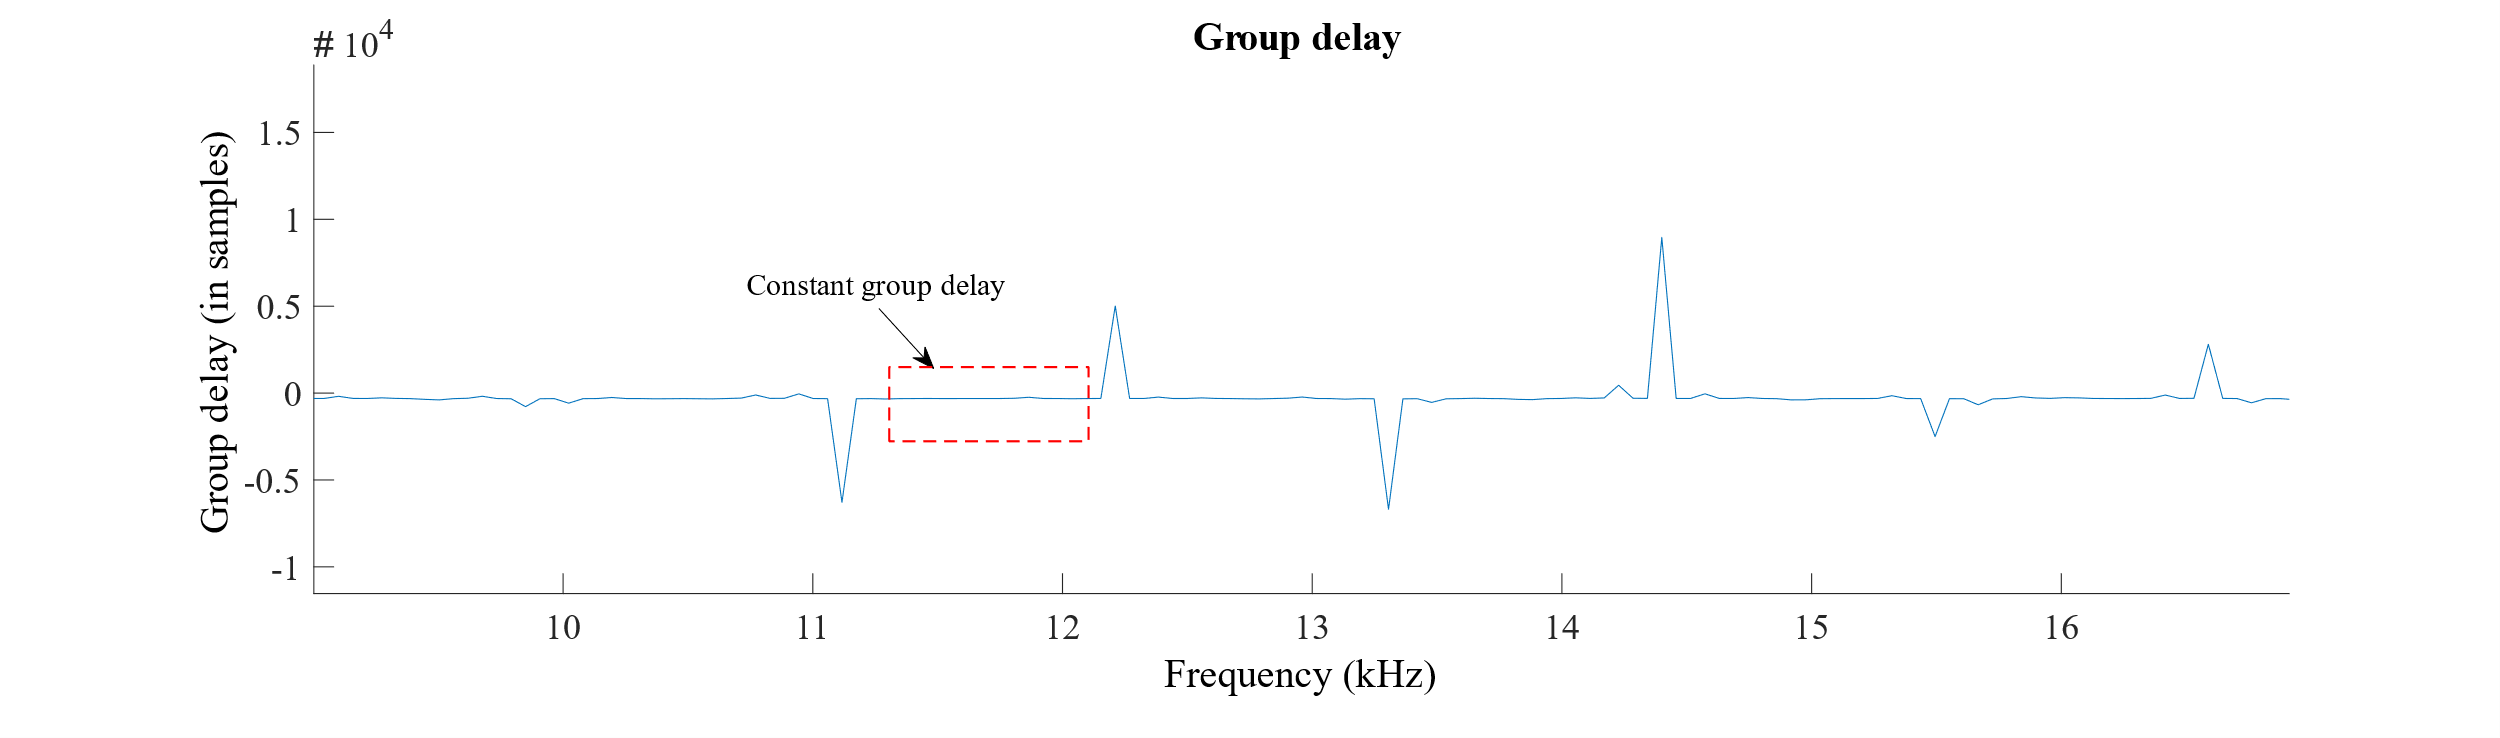
\includegraphics[width=6.44in,height=2.42in]{22}
		\caption{Group delay response}
		\label{fig:_8_Group_delay_response}
	\end{Center}
\end{figure}


%%%%%%%%%%%%%%%%%%%% Figure/Image No: 31 Ends here %%%%%%%%%%%%%%%%%%%%

\par

\par

\begin{justify}
Figure 7.9 represents the phase delay (with respect to samples), it shows also that 11.3-12.2 kHz sampling is the most effective one for the controller.
\end{justify}\par



%%%%%%%%%%%%%%%%%%%% Figure/Image No: 32 starts here %%%%%%%%%%%%%%%%%%%%

\begin{figure}[H]
	\begin{Center}
		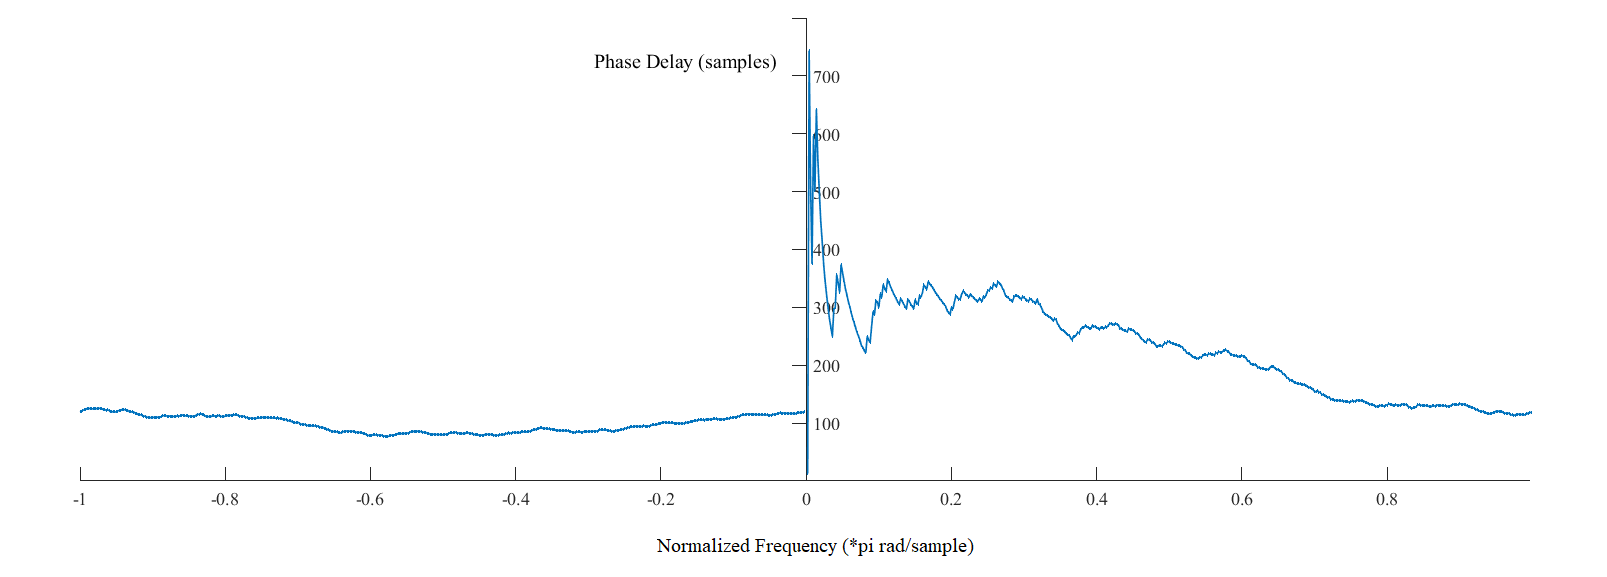
\includegraphics[width=6.5in,height=2.67in]{23}
		\caption{Phase Delay Samples}
		\label{fig:_9_Phase_Delay_Samples}
	\end{Center}
\end{figure}


%%%%%%%%%%%%%%%%%%%% Figure/Image No: 32 Ends here %%%%%%%%%%%%%%%%%%%%

\par

\par


\vspace{\baselineskip}
\begin{justify}
A pole-zero plot shows the location in the complex plane of the poles and zeros of the transfer function of a dynamic system, such as a controller, compensator, sensor, equalizer, filter, or communications channel. ... For a CT system, the plane in which the poles and zeros appear is the s plane of the Laplace transform.
\end{justify}\par



%%%%%%%%%%%%%%%%%%%% Figure/Image No: 33 starts here %%%%%%%%%%%%%%%%%%%%

\begin{figure}[H]
	\begin{Center}
		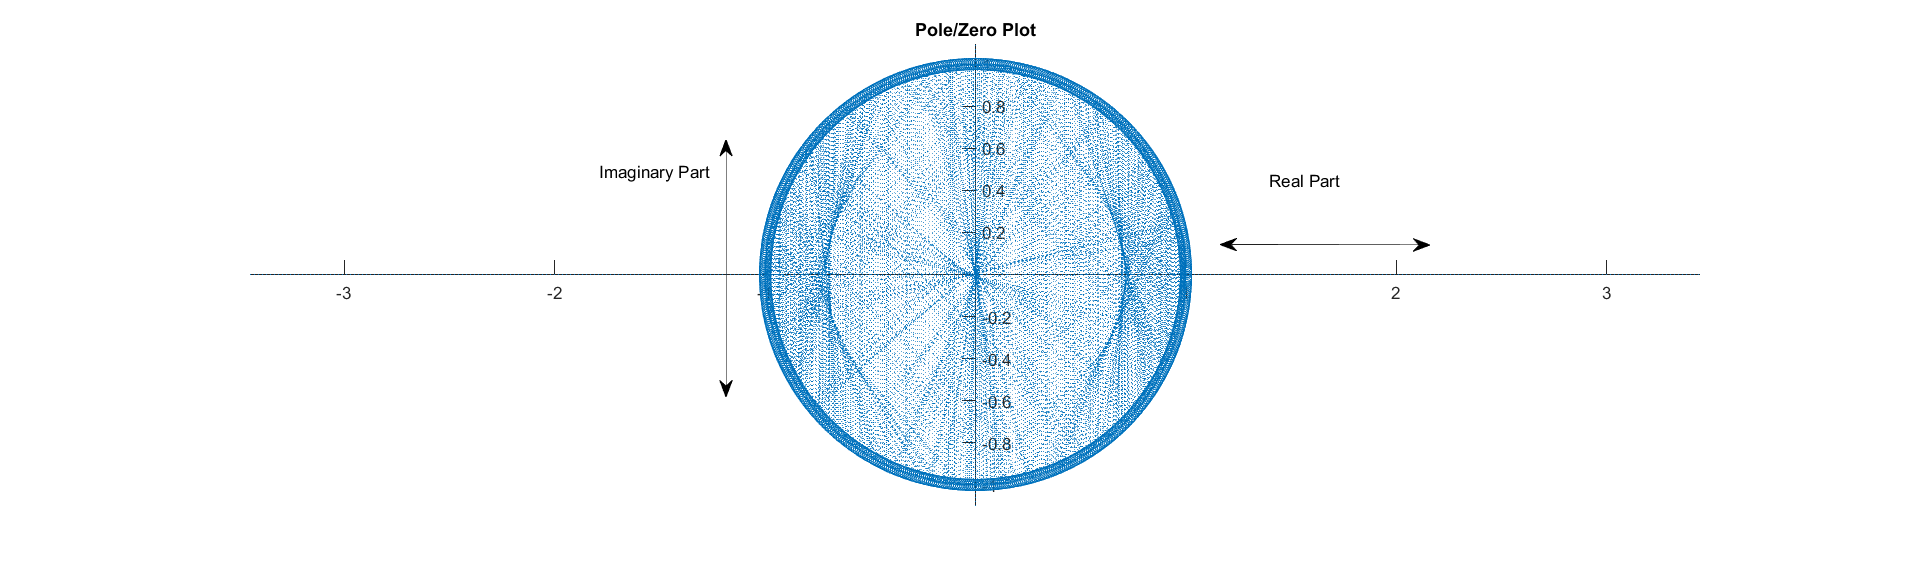
\includegraphics[width=6.55in,height=2.29in]{24}
	\end{Center}
\caption{Pole Zero Plot.}
\end{figure}
Figure 7.10, denotes the pole zero plot for the system, which shows that this system has some noise but ultimately it is stable. Figure 7.11 is the round-off noise power spectrum plot for the system. It shows some unnatural noise in the system.

%%%%%%%%%%%%%%%%%%%% Figure/Image No: 33 Ends here %%%%%%%%%%%%%%%%%%%%

\par

\par


\vspace{\baselineskip}


%%%%%%%%%%%%%%%%%%%% Figure/Image No: 34 starts here %%%%%%%%%%%%%%%%%%%%

\begin{figure}[H]
	\begin{Center}
		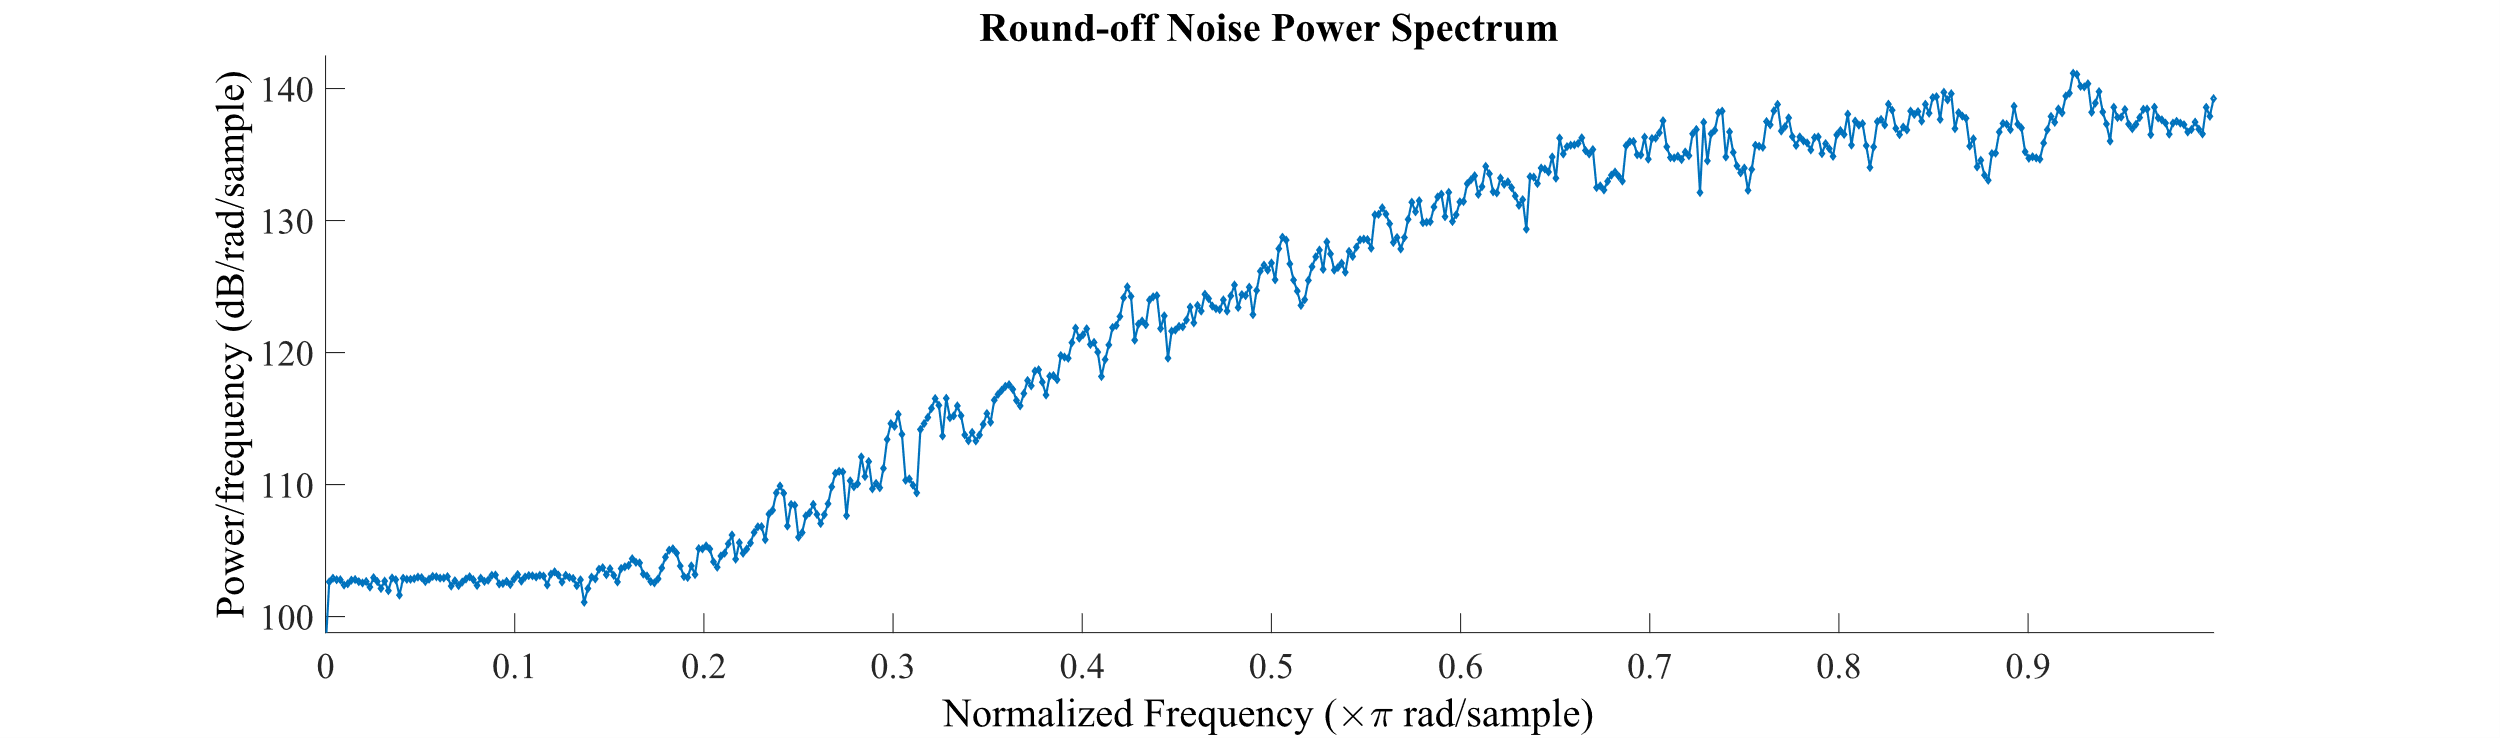
\includegraphics[width=6.46in,height=2.19in]{25}
		\caption{ Round-off noise Power Spectrum.}
		\label{fig:_11_Roundoff_noise_Power_Spectrum}
	\end{Center}
\end{figure}


%%%%%%%%%%%%%%%%%%%% Figure/Image No: 34 Ends here %%%%%%%%%%%%%%%%%%%%
The errors in a fixed-point finite impulse response (FIR) filter due to quantization (analog-to-digital conversion) and roundoff are considered. Expressions for the exact moments of the filter output noise are derived. It is well known that, when the input signal satisfies certain conditions, the popular additive white noise model can be valid in describing the quantization noise. The characteristics of multiplicative roundoff noises, however, differ from what this model predicts, even under conditions where the roundoff noises are white. Hence the additive white noise model does not provide accurate results on the characteristics of the output error in an FIR filter. Using the exact formulas for the moments, the author computes the exact power spectrum of the filter output error. These results agree well with those obtained from simulation.
\par

\par



\vspace{\baselineskip}


%%%%%%%%%%%%%%%%%%%% Figure/Image No: 35 starts here %%%%%%%%%%%%%%%%%%%%

\begin{figure}[H]
	\begin{Center}
		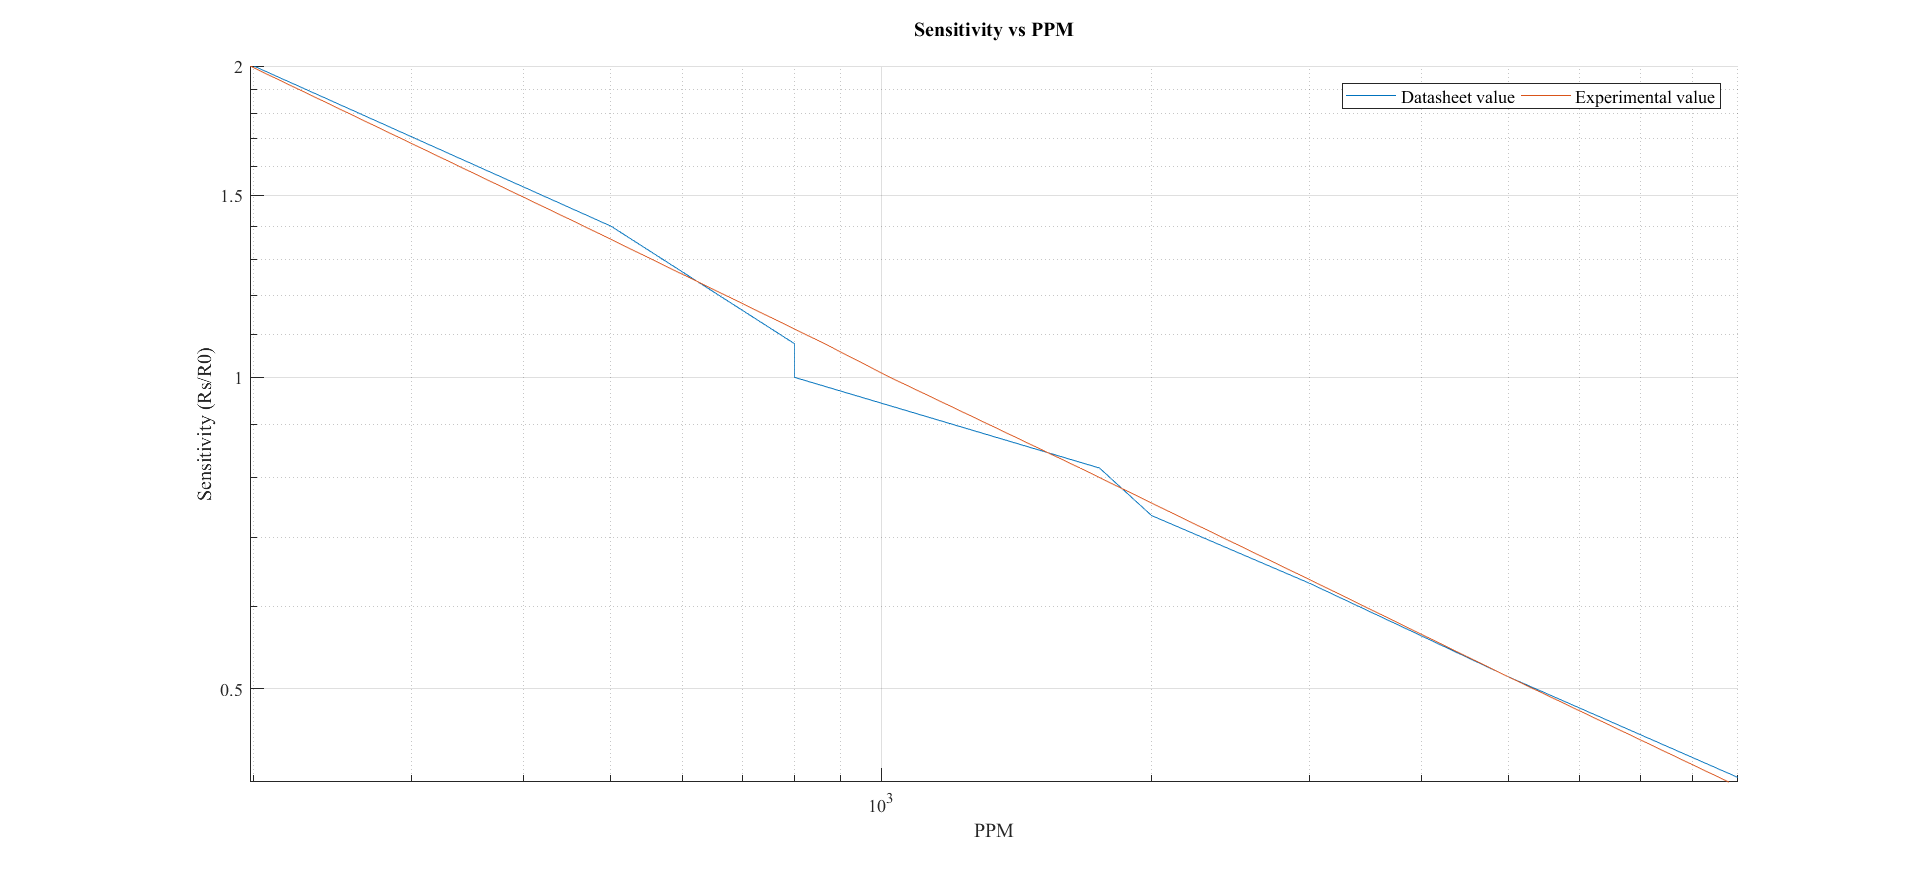
\includegraphics[width=6.42in,height=3.33in]{26}
		\caption{Sensitivity vs PPM graph. (Log-Log plot)}
		\label{fig:_12_Sensitivity_vs_PPM_graph_LogLog_plot}
	\end{Center}
\end{figure}


%%%%%%%%%%%%%%%%%%%% Figure/Image No: 35 Ends here %%%%%%%%%%%%%%%%%%%%

\par

\par
\begin{justify}
Figure 7.12 shows the actual $\&$  experimental Sensitivity vs Concentration plot, from where it can be said that the calibration was 90-95$\%$  accurate, which is good.
\end{justify}\par

\vspace{\baselineskip}


%%%%%%%%%%%%%%%%%%%% Figure/Image No: 36 starts here %%%%%%%%%%%%%%%%%%%%

\begin{figure}[H]
	\begin{Center}
		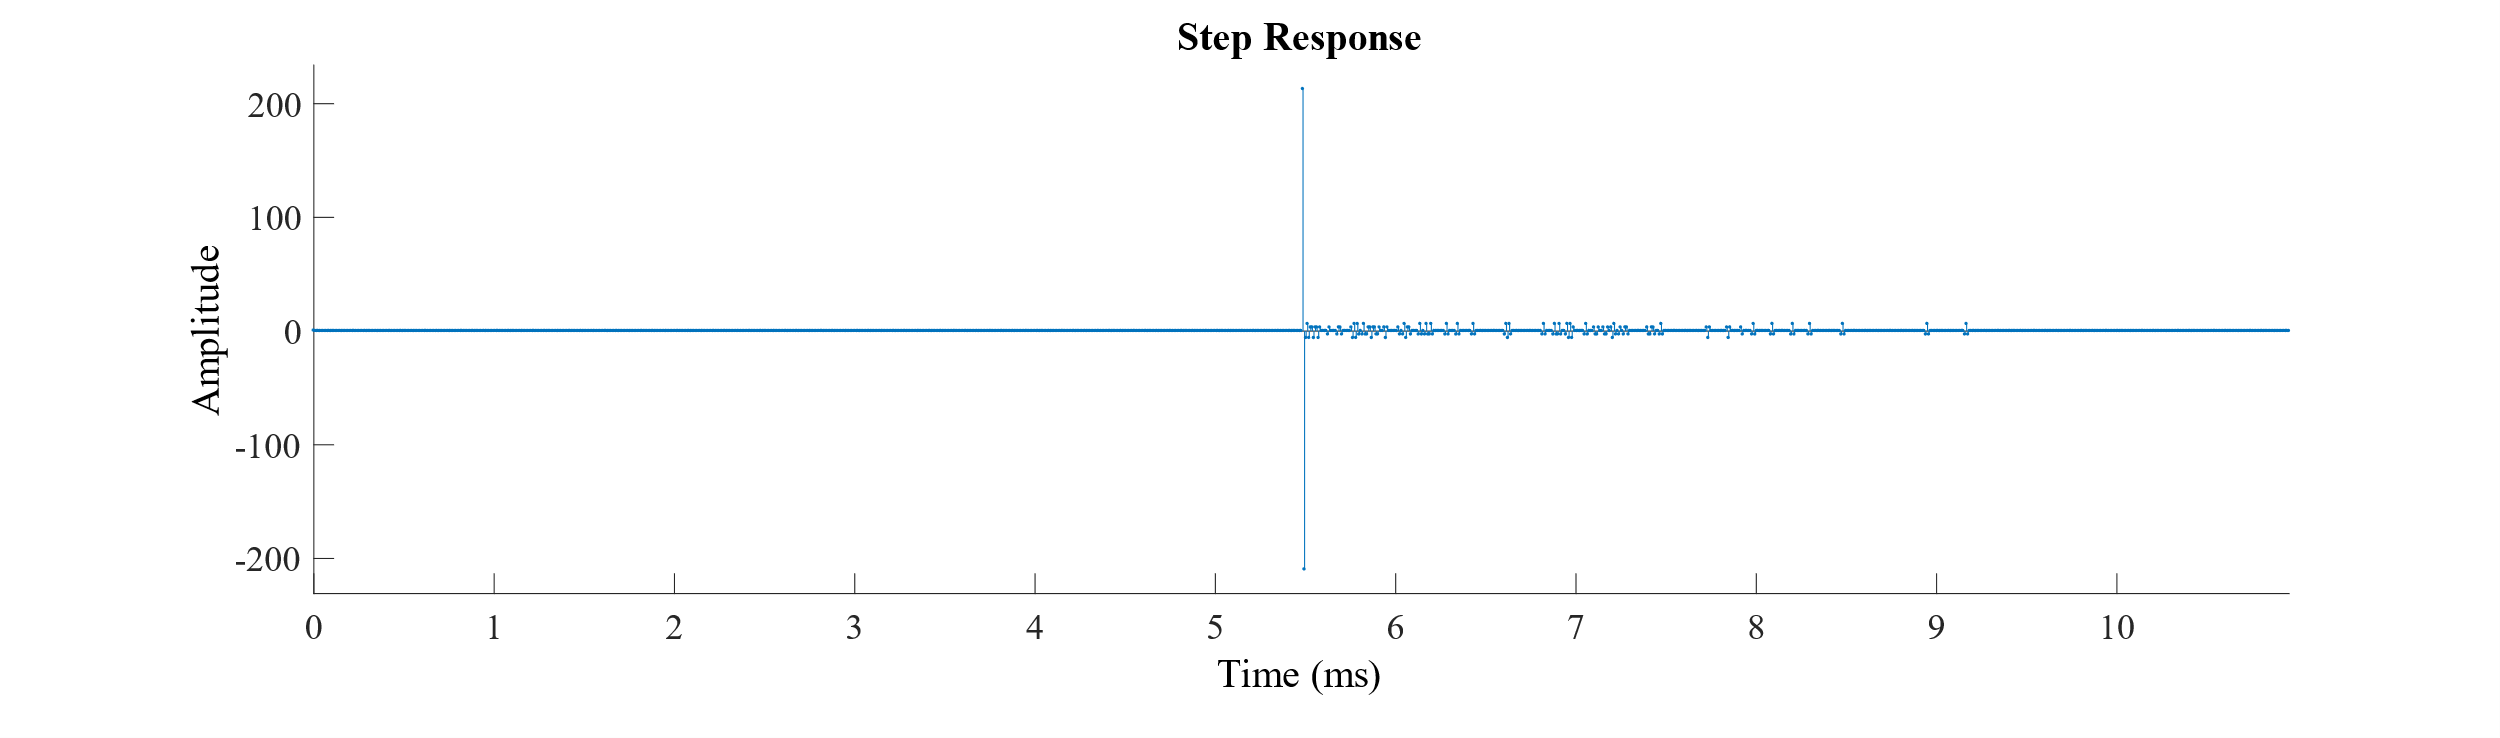
\includegraphics[width=6.5in,height=2.22in]{27}
	\end{Center}
\caption{Step response.}
\end{figure}


%%%%%%%%%%%%%%%%%%%% Figure/Image No: 36 Ends here %%%%%%%%%%%%%%%%%%%%

\par

\par

\begin{justify}
From, Figure 7.13, the step response can be shown where it is seen that initially the system runs fine but after a certain period it shows some abrasions but the used filter automatically fixes the errors. The below, Figure 7.14 shows the time domain and frequency domain analysis plot for the system.
\end{justify}\par



%%%%%%%%%%%%%%%%%%%% Figure/Image No: 37 starts here %%%%%%%%%%%%%%%%%%%%

\begin{figure}[H]
	\begin{Center}
		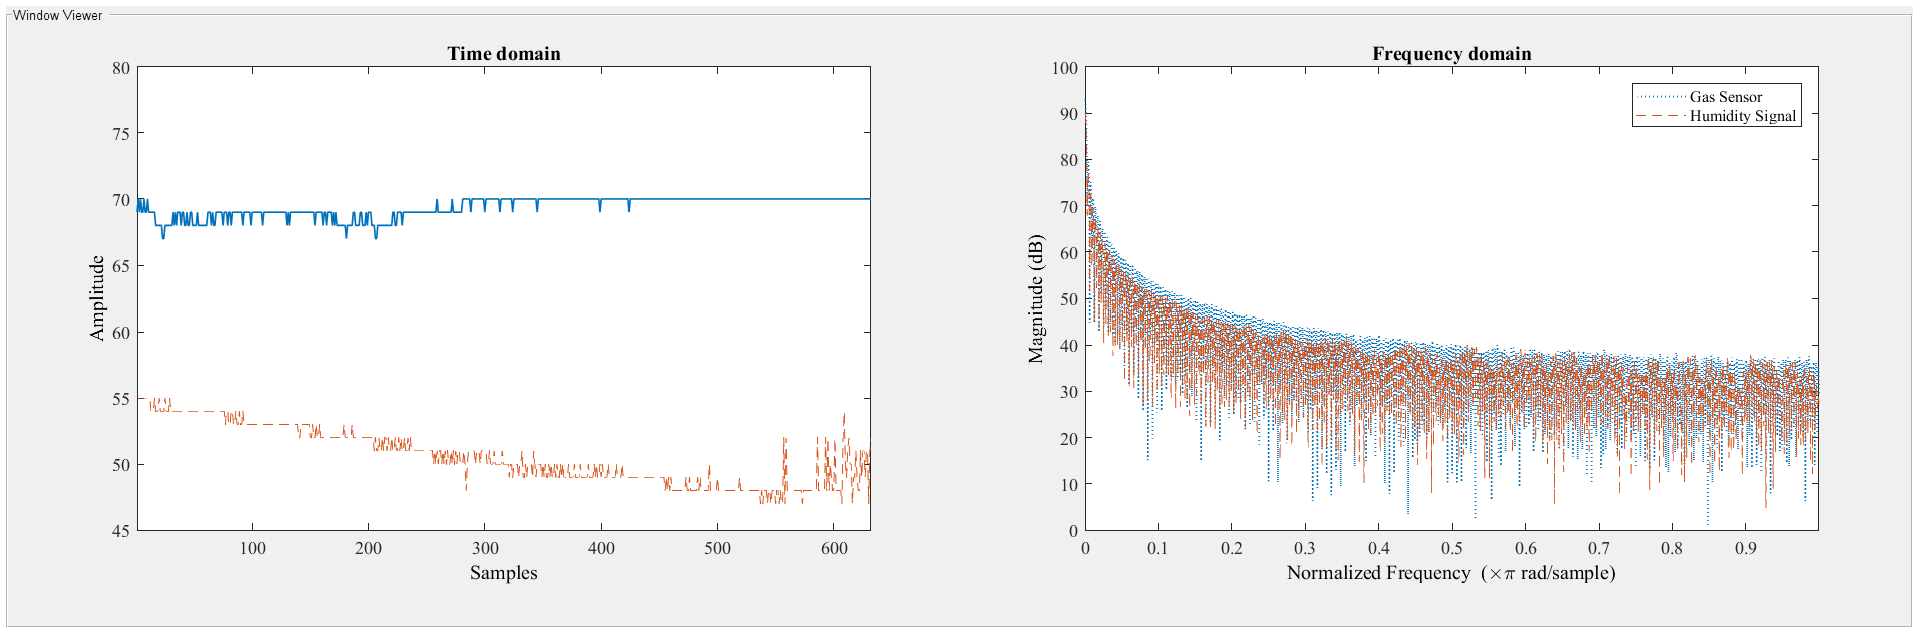
\includegraphics[width=6.53in,height=2.27in]{28}
		\caption{Time domain and Frequency domain graph for the system.}
		\label{fig:_14_Time_domain_and_Frequency_domain_graph_for_the_system}
	\end{Center}
\end{figure}


%%%%%%%%%%%%%%%%%%%% Figure/Image No: 37 Ends here %%%%%%%%%%%%%%%%%%%%

\par

\par

\begin{justify}
The transfer function of the system can be estimated by using Welch Transfer function distribution theory, which is plotted on Figure 7.15. The Figure 7.16 shows the experimental relation between supplied voltage and gas concentration.
\end{justify}\par



%%%%%%%%%%%%%%%%%%%% Figure/Image No: 38 starts here %%%%%%%%%%%%%%%%%%%%

\begin{figure}[H]
	\begin{Center}
		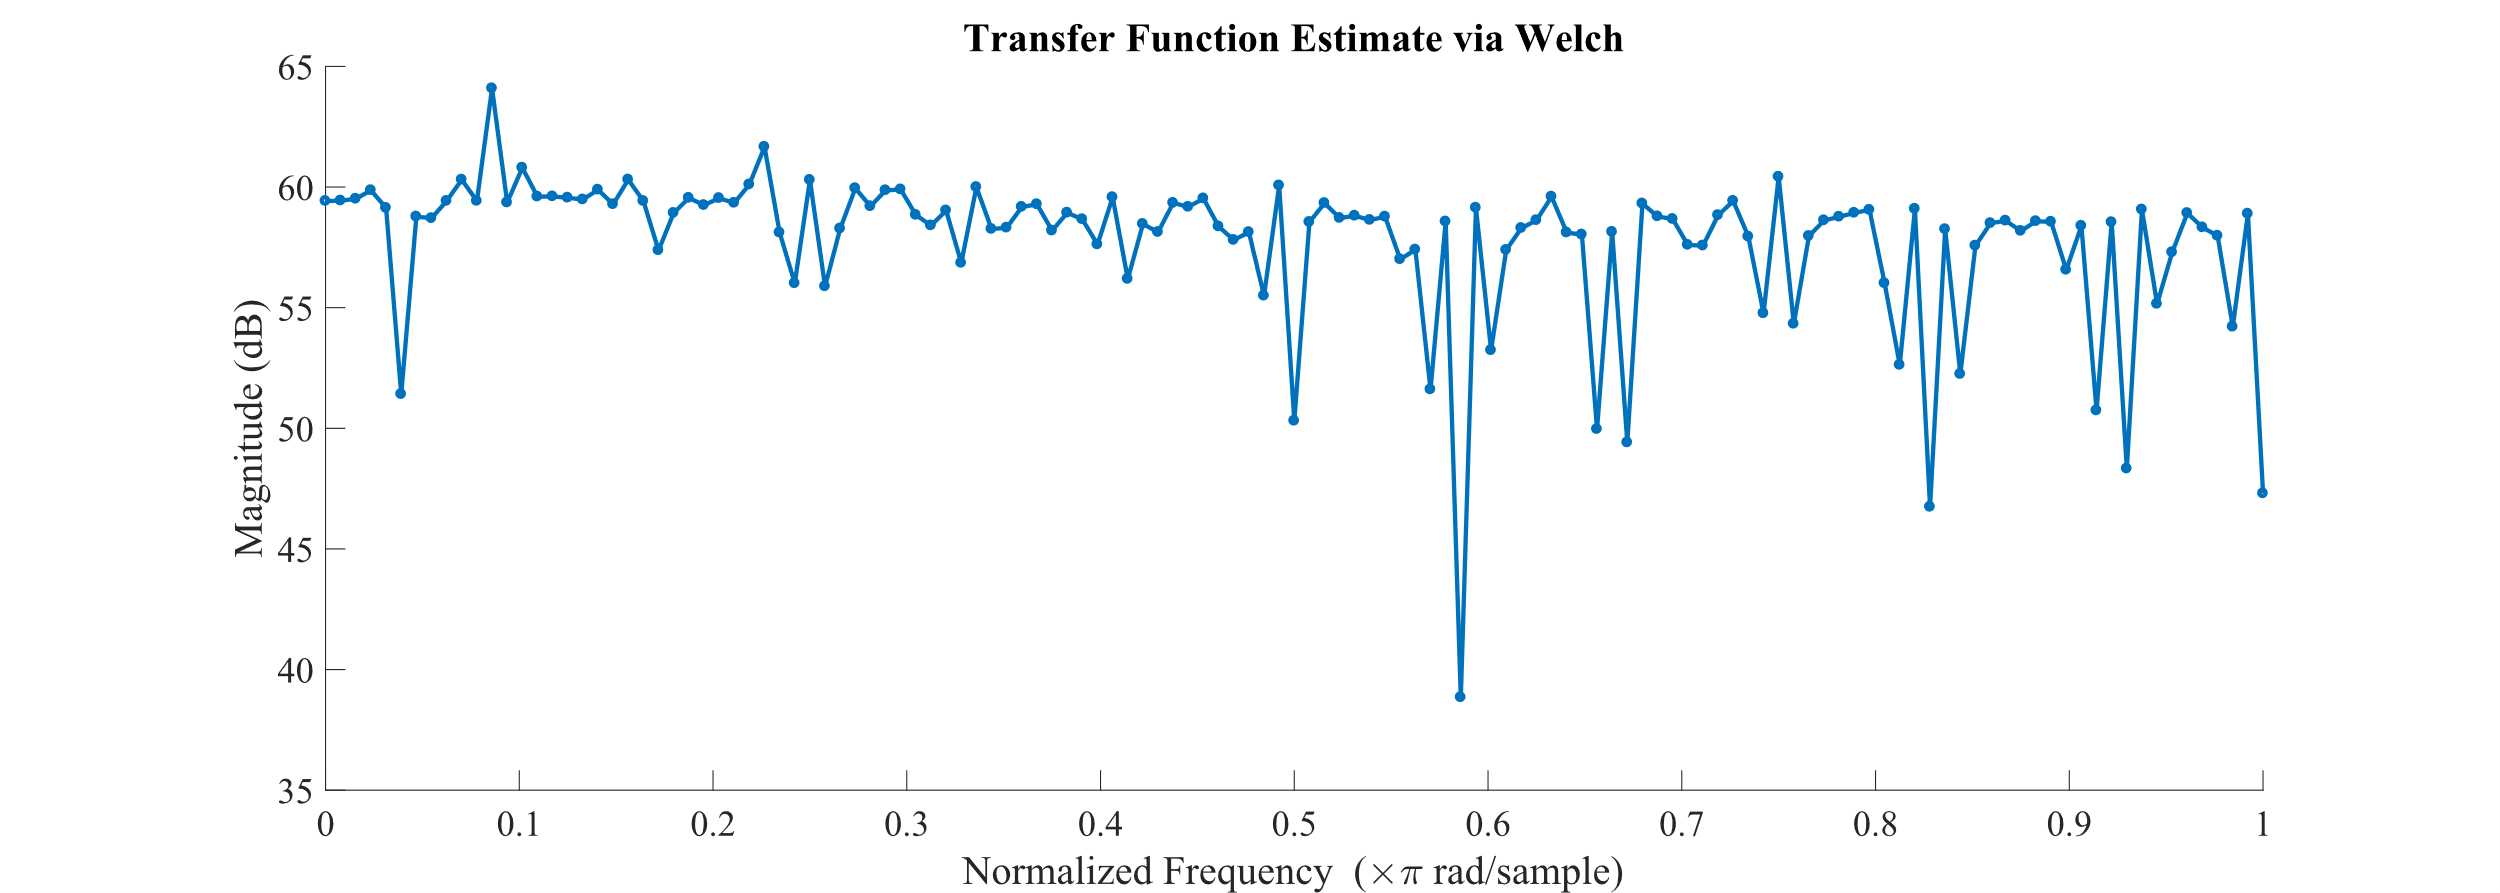
\includegraphics[width=6.51in,height=2.44in]{29}
		\caption{Transfer function estimation via Welch distribution.}
		\label{fig:_15_Transfer_function_estimation_via_Welch_distribution}
	\end{Center}
\end{figure}


%%%%%%%%%%%%%%%%%%%% Figure/Image No: 38 Ends here %%%%%%%%%%%%%%%%%%%%

\par

\par


\vspace{\baselineskip}


%%%%%%%%%%%%%%%%%%%% Figure/Image No: 39 starts here %%%%%%%%%%%%%%%%%%%%
%
%\begin{figure}[H]
%	\begin{Center}
%		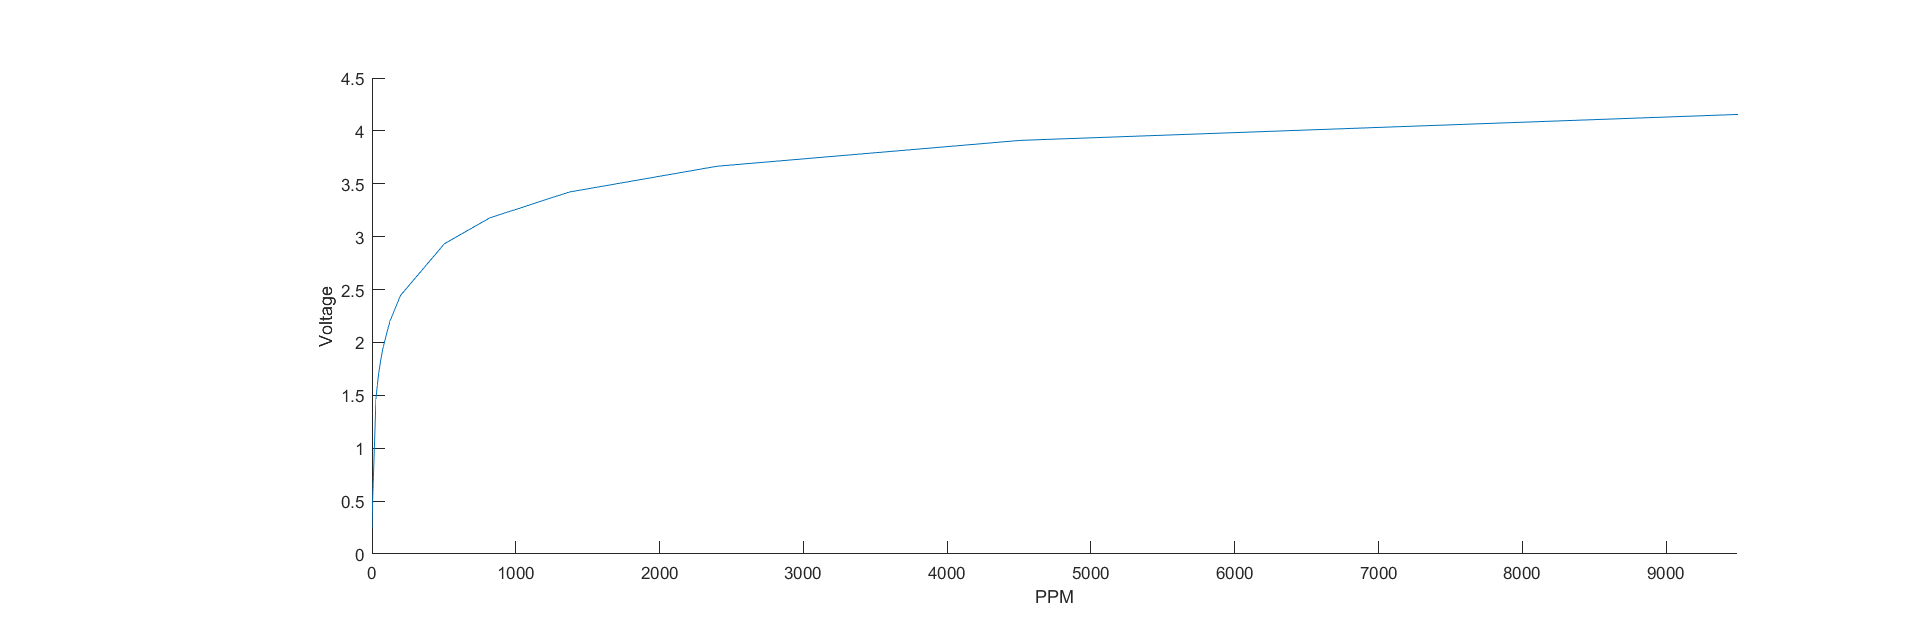
\includegraphics[width=6.37in,height=2.38in]{30}
%		\caption{Voltage vs PPM graph.}
%		\label{fig:_16_Voltage_vs_PPM_graph}
%	\end{Center}
%\end{figure}


%%%%%%%%%%%%%%%%%%%% Figure/Image No: 39 Ends here %%%%%%%%%%%%%%%%%%%%

\par

\par

\item \textbf{Power Spectrum Density Analysis (PSE or PSD):} PSE is most important application area in Digital Signal Processing. There are
mainly two types of power spectrum estimation (PSE) method: Parametric and nonparametric. Parametric or non-classical methods an analyzed process is place by an appropriate model with known spectrum. Non-parametric do not make any assumption on the data generating process. It is start by estimating autocorrelation sequence from a given data. The power spectrum then is estimated via FT of an estimated autocorrelation sequence. Window function is a mathematical function that is zero valued outside of some chosen period. When another unction or waveform or data sequence is multiplied by a window function, the product is also zero-valued outside the period; all that is left is the part where they overlap the observation through the window. It is simple to apply and understand. In this method the frequency of a filter, HD(w) and the corresponding impulse response, hD(n), are related by the inverse Fourier transform \cite{cheikhrouhou2018hybrid,khelifi2018localization,choosaksakunwiboon2018pre}:


\begin{equation}\tag{7.13}
h_{D} ( n ) = \frac{1}{2 \pi } \int _{- \pi }^{ \pi }H_{D} ( w ) e^{iwn}dw
\end{equation}
\begin{justify}
Where HD(w) is frequency response of a filter and hD(n) is corresponding impulse response. The subscript D is used to make a difference between the ideal and practical responses. Here, HD(w) can be obtained from hD(n) by evaluating the inverse Fourier transform. The truncation of hD(n) to a length M-1 is equivalent to multiplying hD(n)by a rectangular window [2] defined as:
\end{justify}\par


\begin{equation}\tag{7.14}
w ( n ) = \{ \begin{array}{ll}
	1,~ \&n=0,1,2, \ldots .. ( M-1 ) \\
	0,~ \&otherwise\\
	\end{array}
\end{equation}
\begin{justify}
And unit impulse response will be:
\end{justify}\par


\begin{equation}\tag{7.15}
h ( n ) =h_{D} ( n ) .w ( n )
\end{equation}

\begin{equation}\tag{7.16}
h ( n ) = \{ \begin{array}{ll}
	h_{D} ( n ) ,~ \&n=0,1,2, \ldots .. ( M-1 ) \\
	0,~ \&otherwise\\
	\end{array}
\end{equation}
\begin{justify}
Frequency domain function in representation of window function is,
\end{justify}\par


\begin{equation}\tag{7.17}
W ( w ) = \sum _{n=0}^{M-1}w ( n ) .e^{-jwn}
\end{equation}
\begin{justify}
The individuality of it play a significant role in establishment of the resulting frequency response of the finite impulse response filter obtained by truncation hD(n) to length M. The undesirable effects are best alleviated by the use of window that do not contain abrupt discontinuities in their time domain characteristics and have likewise low side lobes in their frequency domain characteristics. For the same value of M for both Rectangular and Hamming window or other windows, the width of the main lobe is also wider for these windows compared to the rectangular window. The Fourier transform of rectangular window \cite{movlaee2018microwave,goutham2018flexible,arif2018gait,tischler2018system,sloo2018smart,losey2018review,yilmaz2018pv,he2017adaptive,walczak2019artificial,comer2018internet}:
\end{justify}\par


\begin{equation}\tag{7.18}
W ( w ) = \sum _{n=0}^{M-1}e^{-jwn}
\end{equation}
\begin{justify}
On simplification equation-(7.18) reaches,
\end{justify}\par


\begin{equation}\tag{7.19}
W ( w ) = \sum _{n=0}^{M-1}e^{-jwn}=e^{-jw.\frac{ ( M-1 ) }{2}}.\frac{sin ( wM/2 ) }{sin ( w/2 ) }
\end{equation}
\begin{justify}
The Hamming window function in time domain decrease more gently towards zero on either side and in frequency domain, the amplitude of the main lobes is wider approximately double than that of rectangular window, but side lobes are lesser relative to the main lobe about 40 dB down the main lobes, compared with 14 dB for the rectangular window. Hamming window lead to a filter with wider transition width but higher stopband attenuation.
\end{justify}\par


\begin{equation}\tag{7.20}
Y ( n ) =x ( n ) .w ( n )
\end{equation}
\begin{justify}
Where Y(n) is output signal x(n) is input signal, and w(n) [1] is window function.
\end{justify}\par


\begin{equation}\tag{7.21}
w ( n ) =0.54+0.46cos ( \frac{2 \pi }{N} ) ,~ where \{ \begin{array}{ll}
	-\frac{N}{2} \leq n \leq \frac{N}{2}  ( N=Even number ) \\
	- ( N-2 )  \leq n \leq \frac{ ( N-1 ) }{2} ( N=odd number ) \\
	\end{array}
\end{equation}
\begin{justify}
Transition width,  \(  \Delta f=\frac{3.3}{N} \) . Where N is filter length, and $ \Delta $ \textit{f} is normalized transition width Window Length, L = N+1. In Power Spectrum Estimation is most important application area in Digital Signal Welch method have two basic modification to the normal analytic method. These are allowed the data length to overlap. The data segment can be represented as,
\end{justify}\par


\begin{equation}\tag{7.22}
x ( n ) =x ( n+iD )  \{ \begin{array}{ll}
	n=0,1,2, \ldots  \ldots . ( M-1 ) \\
	i=0,1,2, \ldots  \ldots  \ldots . ( L-1 ) \\
	\end{array}
\end{equation}
\begin{justify}
Where iD is the starting point for the ith sequence. If D = M, the segment does not overlap and the L of data sequence is identical to the data segment of Bartlett method. The second change in Welch method is to window the data segments prior to computing the periodogram \cite{liu2018survey}.
\end{justify}\par


\begin{equation}\tag{7.23}
P_{xx}^{i} ( f ) =\frac{1}{MU} \vert  \sum _{n=0}^{M-1}x ( n ) .w ( n ) .e^{-j.2 \pi fn} \vert , where i=1,2, \ldots  \ldots  \ldots .. ( L-1 )
\end{equation}
\begin{justify}
Where U is a normalization factor for the power.
\end{justify}\par


\begin{equation}\tag{7.24}
U=\frac{1}{M} \sum _{n=0}^{M-1}w^{2} ( n )
\end{equation}
\begin{justify}
The Welch power spectrum estimate is the average of modified periodogram \cite{cheikhrouhou2018hybrid}, is
\end{justify}\par


\begin{equation}\tag{7.25}
P_{xx}^{w}=\frac{1}{L} \sum _{i=0}^{L-1}P_{xx}^{i} ( f )
\end{equation}
\begin{justify}
Mean value of Welch estimate,
\end{justify}\par


\begin{equation}\tag{7.26}
E [ P_{xx}^{w} ( f )  ] =\frac{1}{L} \sum _{i=0}^{L-1}E.P_{xx}^{i} ( f )
\end{equation}
\begin{justify}
The resolution of estimated power estimation is determined by the spectral resolution of each segment which is of length L, it is window dependent. From equations-(7.25) to (7.26), Figure 7.16 $\&$  Figure 7.17 can be drawn \cite{chatterjee2018artificial}.
\end{justify}\par



%%%%%%%%%%%%%%%%%%%% Figure/Image No: 40 starts here %%%%%%%%%%%%%%%%%%%%

\begin{figure}[H]
	\begin{Center}
		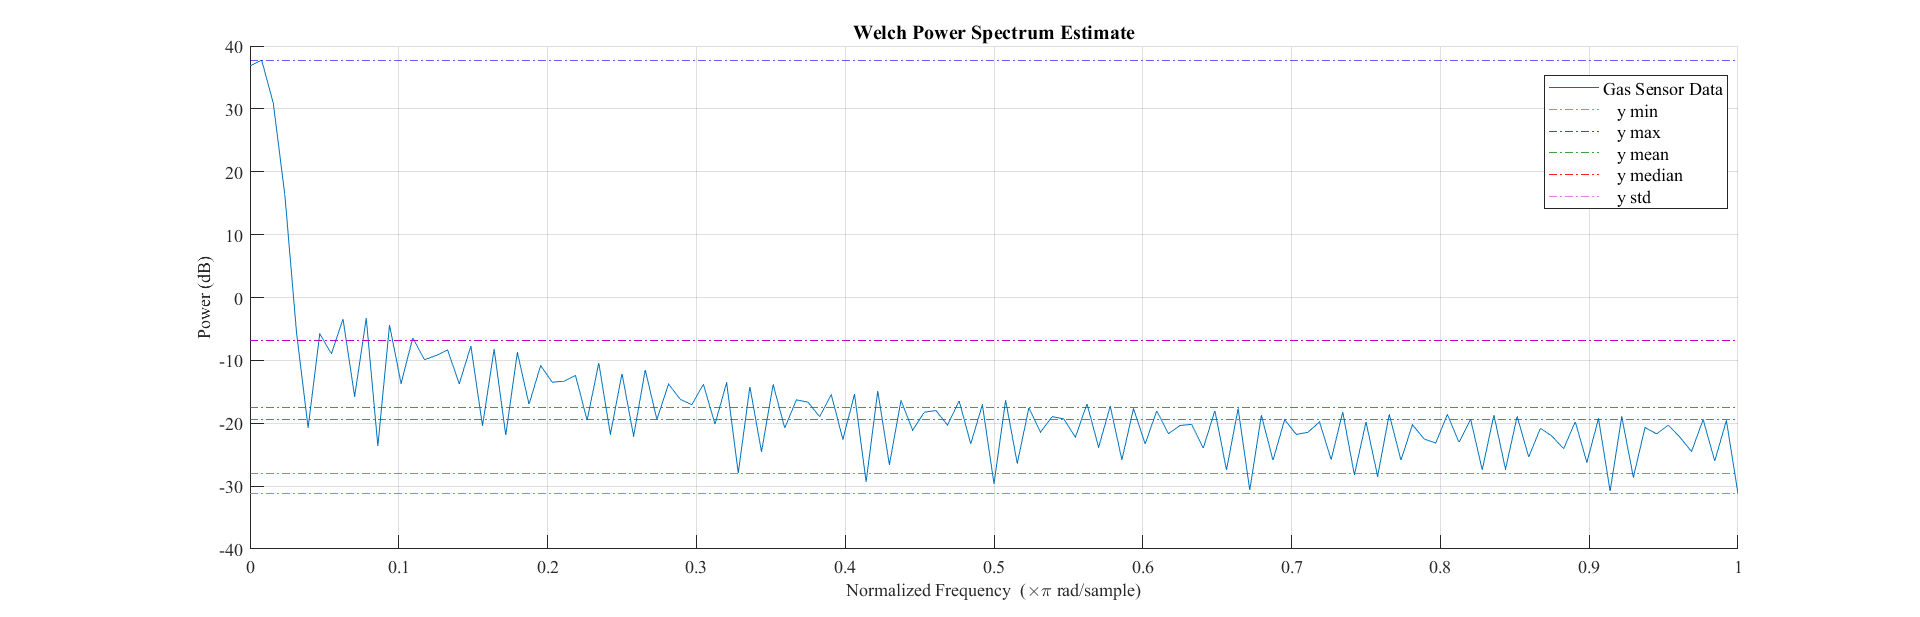
\includegraphics[width=6.61in,height=2.4in]{31}
		\caption{Welch power spectrum estimate for Gas sensor.}
		\label{fig:_17_Welch_power_spectrum_estimate_for_Gas_sensor}
	\end{Center}
\end{figure}


%%%%%%%%%%%%%%%%%%%% Figure/Image No: 40 Ends here %%%%%%%%%%%%%%%%%%%%

\par

\par


\vspace{\baselineskip}


%%%%%%%%%%%%%%%%%%%% Figure/Image No: 41 starts here %%%%%%%%%%%%%%%%%%%%

\begin{figure}[H]
	\begin{Center}
		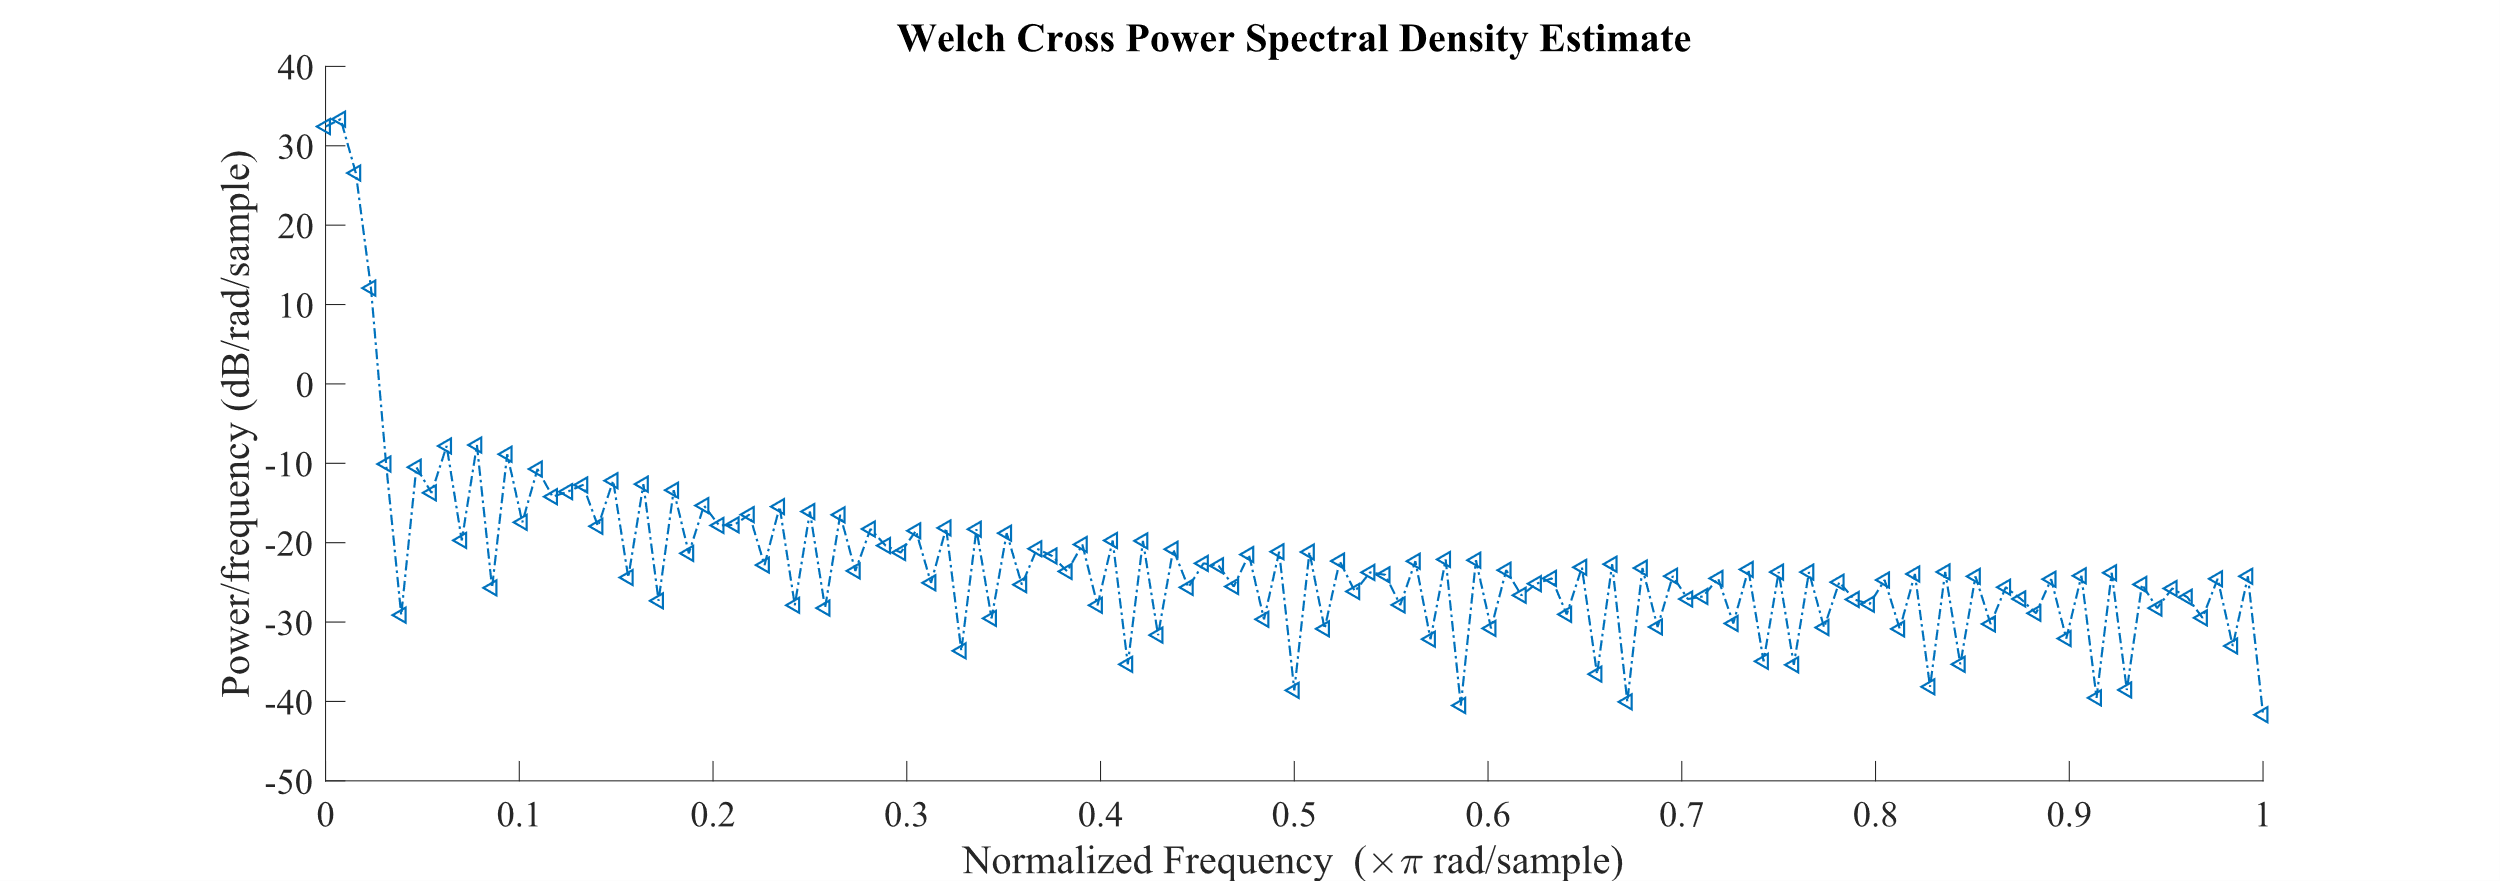
\includegraphics[width=6.52in,height=2.59in]{32}
	\end{Center}
\caption{Welch Cross power density estimate.}
\end{figure}


%%%%%%%%%%%%%%%%%%%% Figure/Image No: 41 Ends here %%%%%%%%%%%%%%%%%%%%

\par

\par
\end{enumerate}
\setlength{\parskip}{8.04pt}
\section{Feedback Control for the Controller }
\begin{justify}
In this system, the reference value is set at 2000 ppm of smoke concentrations. Whenever the controller gets a reading higher than 2000 ppm from the gas sensor then it automatically activates the actuators and the rise in concentration gets mitigated. Thus, the error in the system is eliminated very soon after it takes place in the plant. Fig. shows the schematic of the used feedback method of control for the proposed system.
\end{justify}\par



%%%%%%%%%%%%%%%%%%%% Figure/Image No: 42 starts here %%%%%%%%%%%%%%%%%%%%

\begin{figure}[H]
	\begin{Center}
		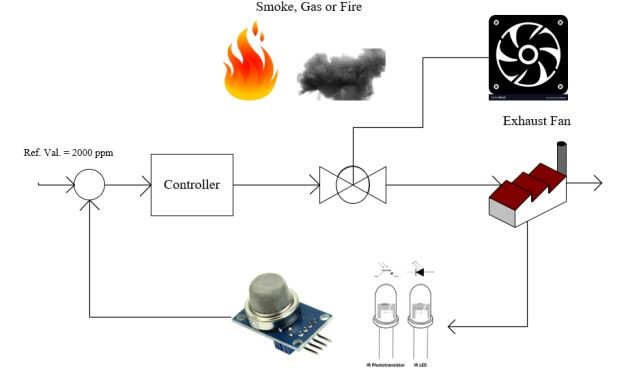
\includegraphics[width=4in,height=2in]{33}
		\caption{Schematic for feedback control system}
		\label{fig:_19_Schematic_for_feedback_control_system}
	\end{Center}
\end{figure}


%%%%%%%%%%%%%%%%%%%% Figure/Image No: 42 Ends here %%%%%%%%%%%%%%%%%%%%

\par

\par

\section{Feedforward Control for the Controller }
\begin{justify}
For the feedforward control, when any abruptions take place in any sensors, then it is very necessary to mitigate the error before it takes place in the plant. Thus, manual wireless switching is introduced here to control the abruptions. From the computer, the actuation signal buttons are pressed from the webpage which in regards sends a signal to the controller via\textit{ }a routing media (for this experiment a 300 mbps router is used). When the signal is received by the controller, a swift actuator switching takes place to mitigate the abruptions. Fig. shows the graphical representation of the proposed feedforward control system for the experimental setup.
\end{justify}\par



%%%%%%%%%%%%%%%%%%%% Figure/Image No: 43 starts here %%%%%%%%%%%%%%%%%%%%

\begin{figure}[H]
	\begin{Center}
		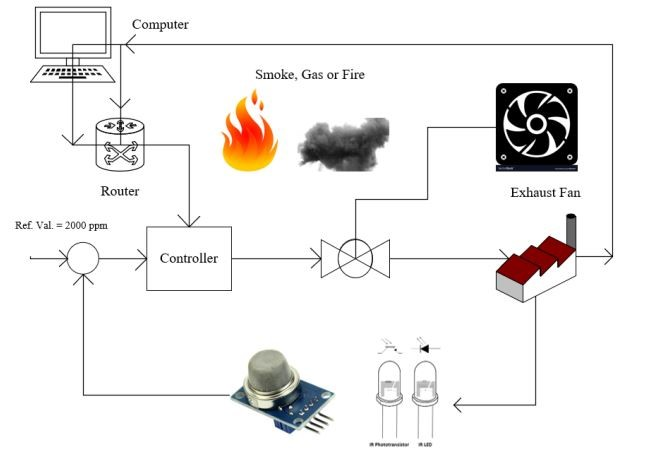
\includegraphics[width=4in,height=2in]{34}
		\caption{Schematic for feedforward control system}
		\label{fig:_20_Schematic_for_feedforward_control_system}
	\end{Center}
\end{figure}


%%%%%%%%%%%%%%%%%%%% Figure/Image No: 43 Ends here %%%%%%%%%%%%%%%%%%%%

\par

\par
\newpage

\vspace{\baselineskip}
\section{Data Security }
Data security refers to the process of protecting data from unauthorized access and data corruption throughout its lifecycle. Data security includes data encryption, tokenization, and key management practices that protect data across all applications and platforms.Cloud adoption is increasing risks of data breach, data loss, and non-compliance with data privacy regulations.
\subsection{Cryptographic nonce}
\begin{justify}
A nonce is a random or semi-random number that is generated for a specific use, typically related to cryptographic communication or information technology. The term itself stands for number used once  or number once  and is most commonly referred to specifically as a cryptographic nonce. Data was sent by adding an arbitrary value and when data was received by a controller it subtracted the arbitrary value by itself. The value was randomly selected by the user. If any attack will occur during data communication the attacker will get the data with the added arbitrary value.
\end{justify}\par
\section{Chapter Summery}
In this chapter all test result and data analysis was performed.Data analysis using different types of filtering method and algorithms was also performed in this chapter and data security of the system also explained here for the security purposes.Althouth system stability and performance of the system also be determined in this chapter. 